% options:
% thesis=B bachelor's thesis
% thesis=M master's thesis
% czech thesis in Czech language
% slovak thesis in Slovak language
% english thesis in English language
% hidelinks remove colour boxes around hyperlinks

\documentclass[thesis=B,czech]{FITthesis}[2012/06/26]

\usepackage[utf8]{inputenc} % LaTeX source encoded as UTF-8

\usepackage{graphicx} %graphics files inclusion
% \usepackage{amsmath} %advanced maths
% \usepackage{amssymb} %additional math symbols

\usepackage{dirtree} %directory tree visualisation

% % list of acronyms
% \usepackage[acronym,nonumberlist,toc,numberedsection=autolabel]{glossaries}
% \iflanguage{czech}{\renewcommand*{\acronymname}{Seznam pou{\v z}it{\' y}ch zkratek}}{}
% \makeglossaries

\newcommand{\tg}{\mathop{\mathrm{tg}}} %cesky tangens
\newcommand{\cotg}{\mathop{\mathrm{cotg}}} %cesky cotangens

%%%%%%%%%%%%%%%%%%
% ZACATEK PRACE

\department{Katedra IS}
\title{Webový portál pro podporu výuky na střední škole}
\authorGN{Vladimír} %(křestní) jméno (jména) autora
\authorFN{Mlázovský} %příjmení autora
\authorWithDegrees{Vladimír Mlázovský} %jméno autora včetně současných akademických titulů
\supervisor{Mgr. Monika Součková}
\acknowledgements{Petr Novotný}
\abstractCS{Cílem této práce bylo vytvoření webového portálu pro podporu výuky na střední škole, který je zaměřený především na sdílení výukových materiálů směrem od učitelů k žákům. Učitelé nahrávají své prezentace a písemné práce na webový portál do přehledné a předem nastavené hierarchie. Studenti k těmto materiálům přistupují přes svůj uživatelský účet. Veškerá aktivita je skrze autentizaci – k materiálům není veřejný přístup.}
\abstractEN{The objective of my work is implementing web portal to support education on secondary school. It allows sharing some education materials from teachers to students. Teachers upload their tests and presentations to web into fixed structure. Students open these documents from theirs homes. All activity on this web is after logging - there is not public access.}
\placeForDeclarationOfAuthenticity{V~Praze}
\declarationOfAuthenticityOption{4} %volba Prohlášení (číslo 1-6)
\keywordsCS{webový portál, výuka, střední škola, sdílení studijních materiálů}
\keywordsEN{web portal, education, secondary school, sharing education documents}

\begin{document}

% \newacronym{CVUT}{{\v C}VUT}{{\v C}esk{\' e} vysok{\' e} u{\v c}en{\' i} technick{\' e} v Praze}
% \newacronym{FIT}{FIT}{Fakulta informa{\v c}n{\' i}ch technologi{\' i}}

%%%%%%%%%%%%%%%%%%
%  PRACE

\begin{introduction}
Cílem této práce bylo vytvoření webového portálu pro podporu výuky na střední škole, který je zaměřený především na sdílení výukových materiálů směrem od učitelů k žákům. Učitelé nahrávají své prezentace a písemné práce na webový portál do přehledné a předem nastavené hierarchie. Studenti přistupují k těmto materiálům přes svůj uživatelský účet. Veškerá aktivita je skrze autentizaci – k materiálům není veřejný přístup. Učitelé mají díky statistikám přehled o návštěvnosti svých stránek.

\section{Motivace} 
Tento systém z mé strany otestuje moje znalosti a schopnosti. Navazuji na svoji dřívější práci s novými zkušenostmi, přístupem a znalostí trendů. Tento portál, bude-li postaven tak, jak popisují následující stránky, poskytne důkaz, že jsem se na škole informačních technologií stal tím, kým jsem chtěl v roce 2011 být.

\section{Struktura práce}
Kapitola \textbf{Cíl práce} se věnuje teorii. Porovnává současná řešení, hledá vzory pro nový studijní portál. \textbf{Analýza} připravila jedno konkrétní řešení. Pátrá přímo u zadavatele po vodítkách, aby pro něj byl nový systém co nejlepší. Na konci analýzy byl vypracován a předán návrh uživatelského rozhraní. \textbf{Implementace} popisuje jak byl systém vytvářen a testován. \textbf{Závěr} hodnotí jak se podařilo naplnit závazky vůči zadavateli i vůči sobě samému a pohrává si s budoucím vývojem. Poslední část - \textbf{Přílohy} - nabízí přehled zkratek, návod jak se dostat k repositáři, náhled do zdrojových kódů a uživatelskou příručku.

\end{introduction}

\chapter{Cíl práce}

Cílem této práce bylo reimplementovat stávající systém na Obchodní akademii v Lysé nad Labem. Stávající systém, který byl rovněž mojí prací, nesplňoval nároky na bezpečnost a byl zbytečně uživatelsky složitý. Nový systém proto je šitý na míru OA Lysá, zadavateli.

Na následujících řádkách se dočtete o stávajících systémech včetně toho, který byl nahrazen. V této kapitole jsou rozebrána různá funkční řešení, co se by se z nich dalo použít pro nový portál, a co nakonec bylo implementováno pro OA Lysá.

\section{Existující systémy}

Přestože první verze vycházela skutečně jen z potřeb zákazníka a mého přesvědčení, \textit{že by to tak asi mělo být}, nebyla úplně špatně. Nyní jsem schopen porovnat své řešení s jinými již existujícími řešeními. Mohl jsem si z nich vzít to, co měl systém dle očekávání umět, a udělat to co nejlépe. Poučit se ze stávajících řešení a posunout své o kousek dál.

Nejbližšími řešeními jsou EDUX, Moodle, Dokuwiki a stávající řešení na OA Lysá. Všechny čtyři jsou v této kapitole rozebrány.

\subsection{EDUX}
Systém pro podporu procesu výuky \cite{edux}. Výhody jsou:

\begin{itemize}
	\item Jednotná struktura předmětů
	\item	Řešení klasifikace
	\item Verzování obsahu
	\item Import/export dat a uživatelů
\end{itemize}

Nevýhodou je orientace na systém výuky na vysokých školách. Z tohoto systému byla přebrána pevná struktura.

Tento systém je skutečně komplexní velmi dobře funkční řešení. Je již od návrhu postaven pro ČVUT FIT a FEL. Právě tento systém mi byl hlavní inspirací.

\subsection{Moodle}
Moodle je volně stažitelný balíček pro tvorbu výukových prezentací a elektronických kurzů. Po stažení základního prostředí se zbytek funkčnosti utváří přidáváním a odebíráním modulů \cite{moodle}. Výhodami jsou:

\begin{itemize}
	\item Integrované šablony
	\item Snadná rozšiřitelnost pomocí modulů
	\item Enterprise řešení a podpora
\end{itemize}

Nevýhodami je, že v Moodlu není možné držet pevnou strukturu menu a větší náročnost při provozu. Navíc OA Lysá by většinu pokročilých funkcí nevyužívala.

Moodle má dobře zpracované testy a možnosti jednorázových akcí. Ani jedno však OA nevyžaduje.

\subsection{Dokuwiki}
Dokuwiki je volně stažitelný a pro programátoy velmi jednoduchý glosář. V tomto řešení se velmi snadno tvoří dokumentace \cite{dokuwiki}. Výhodami jsou:

\begin{itemize}
	\item Jednoduchá syntaxe při tvoření obsahu
	\item Není potřeba databáze
	\item Wiki je velmi dobře čitelná i pouze v textové formě (třeba z příkazové řádky)
	\item Verzování obsahu
\end{itemize}

Nevýhodou je, že ani ve wiki není možné udržet pevnou strukturu menu a spravovat mnoho účtů v různých rolích.

Silnou stránkou Dokuwiki je jednoduchost.

\subsection{Stávající systém}
Stávající systém umožňuje funkce, které v novém budou cíleně potlačeny. Například je možné zvlášť řešit menu a stránky. Podle terminologie webu: zvlášť vytvářet položky menu a k nim pak přiřazovat listy. Dále je možné dělat v podstatě neomezeně hlubokou strukturu menu. Nahrané soubory se vkládaly přes speciální tagy, bylo možné vkládat do libovolné stránky libovolné otevřené PDF a obrázky jak z interní databáze, tak odkazem odkudkoliv z webu. Každý učitel mohl řešit uživatelské účty. Výhody stávajícího řešení:

\begin{itemize}
	\item Velmi malá náročnost na provoz webu
	\item Možnost vkládat do textu otevřený PDF dokument
	\item Po tři roky funkční řešení
\end{itemize}

Obrovskou nevýhodou je velmi špatné zabezpečení. Pomocí odkazů se daly veškeré soubory stahovat. Další nevýhodou je zbytečně složitá práce s menu a listy. Kvůli volnosti vznikaly na webu nepřehledné a zbytečně velmi hluboké struktury. Navíc není možné pohodlně prohlížet web na menší obrazovce chytrého telefonu nebo tabletu.

Naopak je elegantní způsob zapisování listů - pomocí kódu vzdáleně podobného Dokuwiki. Ani ten však nebyl ve škole všeobecně přijat.

\subsection{Závěr}

Výsledkem mé práce je systém, který nepřináší žádnou velkou inovaci, ale je ušitý na míru výuce na netechnické střední škole, jakou OA Lysá je. Systém by měl být ze strany učitele dostatečně jednoduchý, aby do systému mohl přidávat materiály každý z nich. Aby vytvoření stránky bylo podobné něčemu, co dobře znají, třeba odesílání emailové pošty. Systém by měl být dostatečně jednoduchý i ze strany studentů, aby na několik kliknutí nalezli informace, pro které web navštívili. Pro splnění těchto cílů si portál bere z již známých řešení několik vzorů. Strukturu z EDUX a jednoduchost z Dokuwiki.

%%%%%%%%%%%%%%%%%%%%%%%%%%%%%%%%%%%%%%%

\chapter{Analýza}

\section{Požadavky zadavatele OA Lysá nad Labem}

Obchodní akademie Lysá nad Labem původně potřebovala systém pouze kvůli matematice. Účelem mělo být sdílení dříve napsaných písemných prací. Avšak po přednesení návrhu celému učitelskému sboru se nápad rozšířil o využití i na další předměty.

\subsection{Funkční požadavky}

Funkční požadavky  jsou:

\begin{itemize}

	\item Uživatelské účty a jejich správa
	\begin{itemize}
		\item Role: administrátor, učitel, žák, prohlídka, zablokovaný účet, guest
	\end{itemize}

	\item Pevná hierarchie menu
	\begin{itemize}
		\item Předmět - ročník - téma
	\end{itemize}
	
	\item Možnost vkládání a editací
	\begin{itemize}
		\item Obrázky, PDF a jiné dokumenty (pouze vkládání)
		\item Textový WYSIWYG editor
	\end{itemize}

	\item Rozesílání hromadné elektronické pošty
	\item Záznam statistických údajů o návštěvnosti
	\item Diskuze pod jednotlivými tématy
\end{itemize}

\subsection{Nefunkční požadavky}

Nefunkční požadavky jsou:

\begin{itemize}

	\item Webový portál poběží na stejném serveru jako prezentační web školy.
	\item Programovací jazyk PHP/Nette
	\item Úložiště MySQL, souborový systém
	\item Systém musí fungovat i při přihlášení všech studentů (přibližně 200 lidí).
	\item Systém může být v případě aktualizace nebo údržby odstaven.
	\begin{itemize}
		\item Při plánované odstávce je zanechána zpráva na běžné adrese webu.
	\end{itemize}	
	\item Přístup k jakýmkoliv materiálům pouze přihlášenými a oprávněnými uživateli.

\end{itemize}

\section{Uživatelské rozhraní}

V rámci předmětu Tvorba uživatelského rozhraní byl ve čtyřčlenném týmu (Karolína Běhalová, Jan Ševela a Jakub Peták) vypracován návrh uživatelského rozhraní v podobě wireframes.

\subsection{Anketa}

Žákům byla zadána anketa, kterou online vyplnilo více než 40 žáků. V anketě jsme se ptali především na nové funkce a spokojenost se současnou verzí webu. Z ankety vyplynulo, že žáci jsou s webem a jeho aktuální funkcionalitou spokojení (viz obrázek \ref{fig:anketa1}). Ocenili by, kdyby mohli na webu sledovat své známky a také přispívat do některých částí webu podobně jako učitelé (viz obrázek \ref{fig:anketa2}). Ve volné otázce odpovídali žáci takto.

\begin{figure}
  \centering
	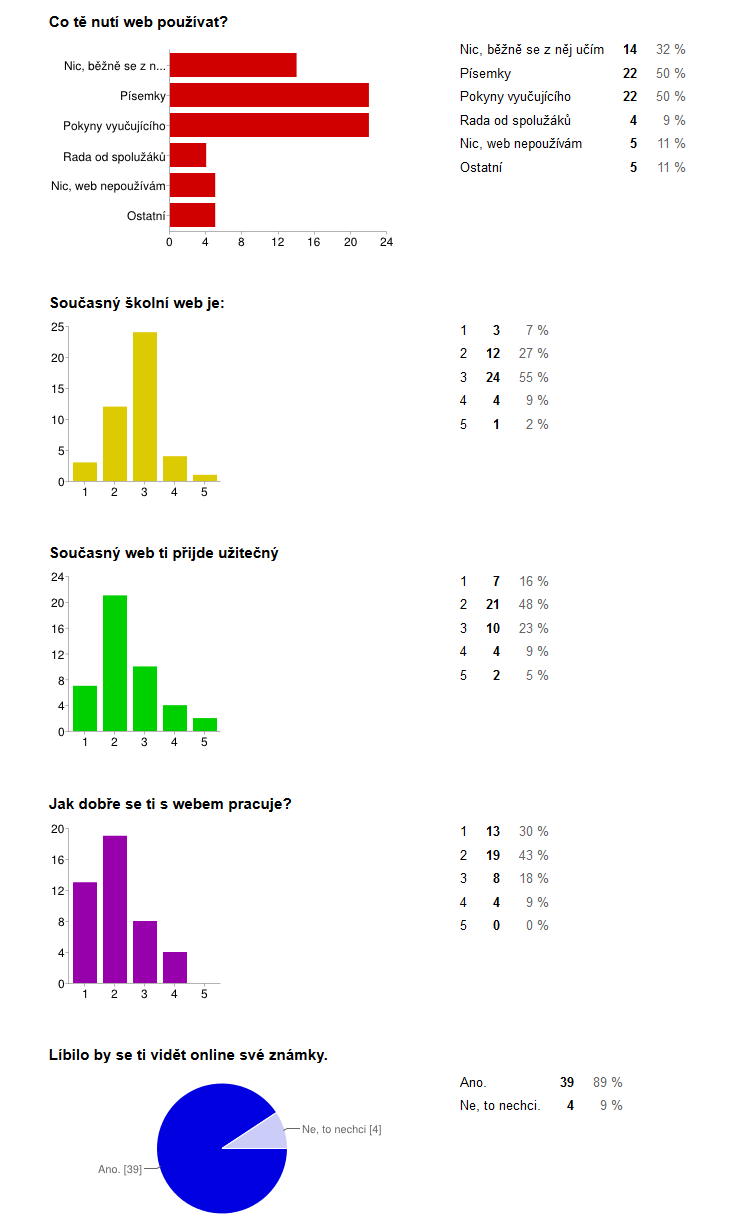
\includegraphics[scale=1.2]{anketa1.png}
	\caption{Výsledky anktery 1. část} \label{fig:anketa1} 
\end{figure}

\begin{figure}
  \centering
	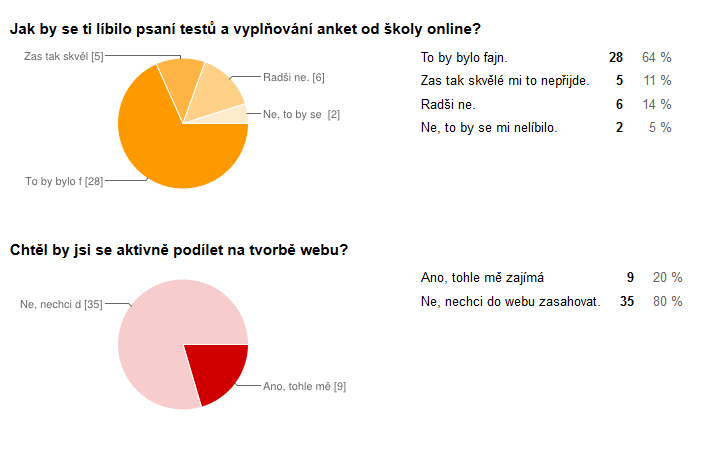
\includegraphics[scale=1.2]{anketa2.png}
	\caption{Výsledky anktery 2. část} \label{fig:anketa2} 
\end{figure}


\uv{Web používám při vypracování domácích úkolů}

\uv{Na webu mi chybí známkování.}

\uv{Uvítala bych jednoznačně větší přehlednost stránek.}

\uv{Rád bych si nastavil vlastní oblíbené položky.}

\subsection{Typy webových stránek}
Každý typ webové stránky bude mít vlastní presenter:

\begin{itemize}
	\item Homepage (loginPage)
	\item Dashboard (home)
	\item Statisticky významné seznamy
	\begin{itemize}
		\item Poslední navštívené
		\item Nejnavštěvovanější
		\item Nejnovější
	\end{itemize}
	\item 	Ročník
	\item Téma
	\item Editace témat
	\item Správa účtů
	\item ...
\end{itemize}

\subsection{Wireframe}

Wireframe\footnote{Celý interaktivní wireframe je na \url{ https://moqups.com/vml/fY80uLDj/p:aaa1dd772}} je ukázka webových stránek, které jsou pouze maketou. Viz obrázek \ref{fig:wireframepc} Na takové maketě sice nic nefunguje, ale velmi přesně reprezentují finální rozložení ovládacích prvků, procházení scénářů a umožňují se tak přesně domluvit se zadavatelem. Wireframe jsme připravili i pro mobilní telefon. Viz obrázek \ref{fig:wireframemobil1} a \ref{fig:wireframemobil2}.

\begin{figure}
  \centering
	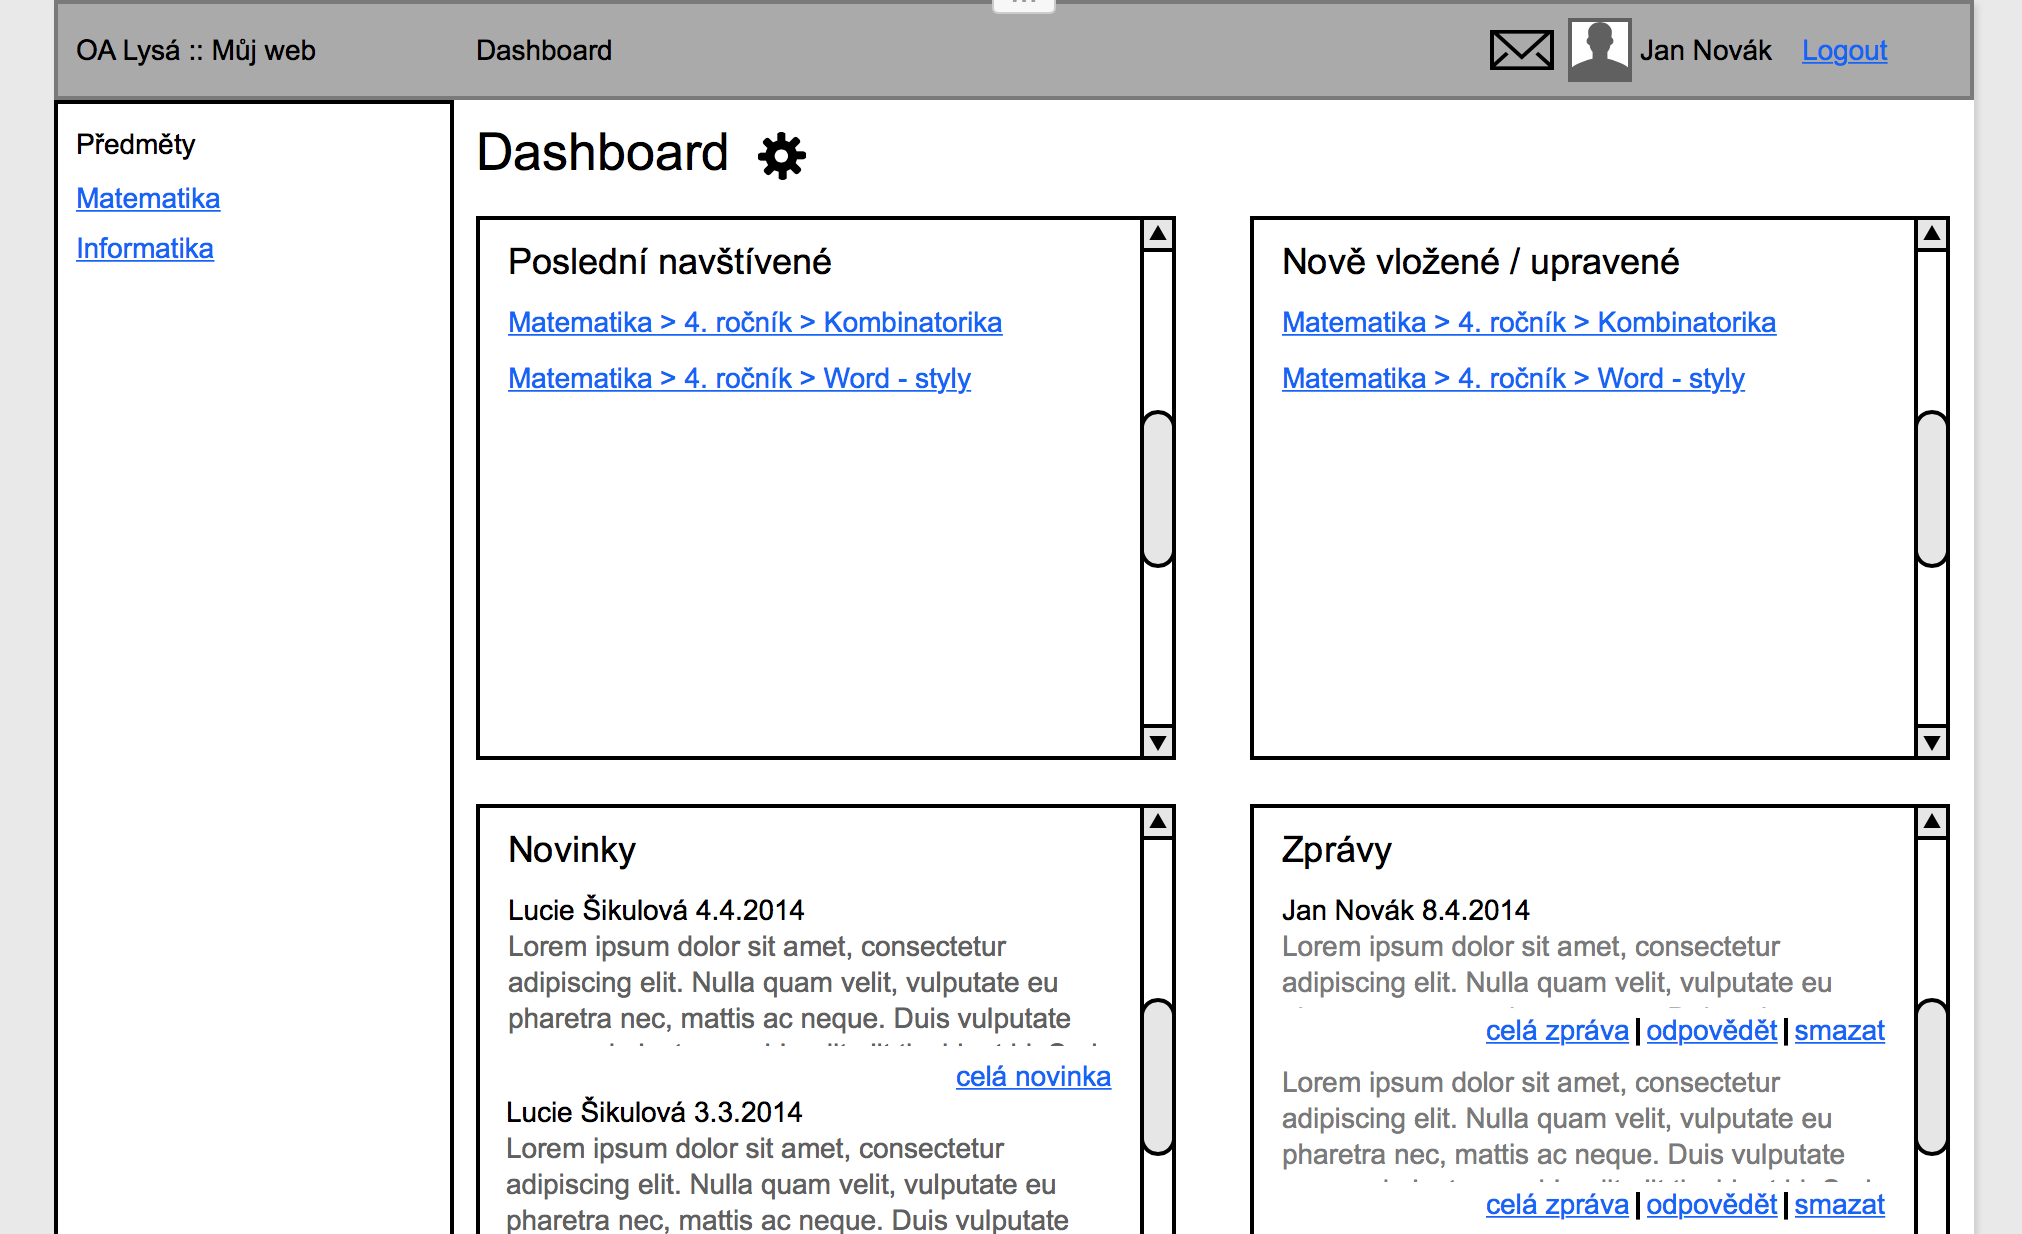
\includegraphics[scale=0.35]{wireframe_desktop_dashboard.png}
	\caption{Wireframe pro PC} \label{fig:wireframepc} 
\end{figure}

\begin{figure}
  \centering
	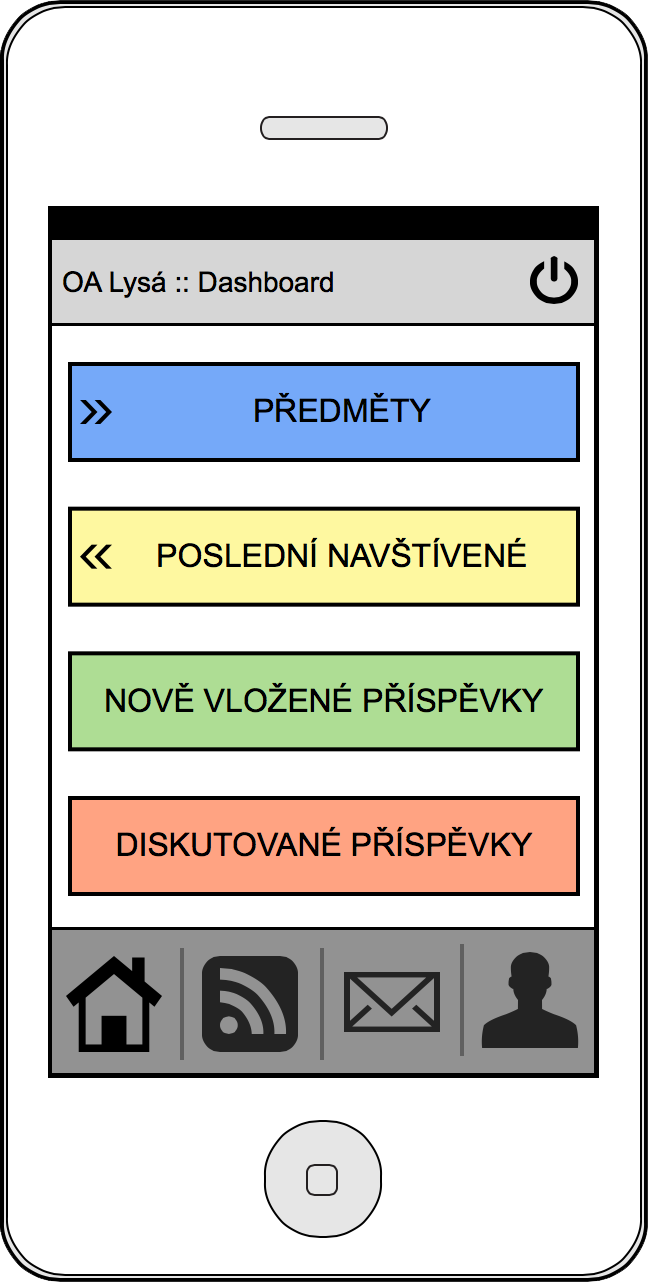
\includegraphics[scale=0.35]{wireframe_phone_dashboard.png}
	\caption{Wireframe pro mobil 1} \label{fig:wireframemobil1} 
	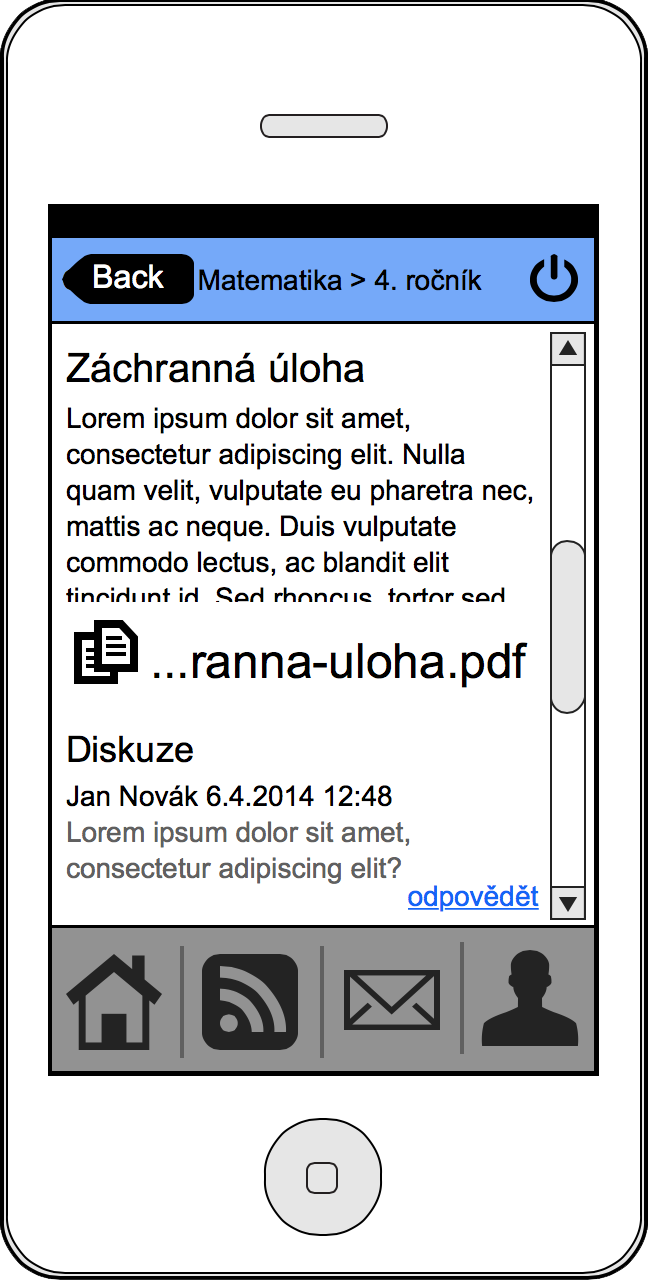
\includegraphics[scale=0.35]{wireframe_phone_tema.png}
	\caption{Wireframe pro mobil 2} \label{fig:wireframemobil2} 
\end{figure}


\section{Cílové skupiny}

Cílové skupiny jsou na webovém portále pro podporu výuky na středních školách dvě. Učitelé a žáci. Nebo by tyto dvě skupiny mohly být pojmenovány redaktoři a čtenáři.

\section{Persony}

Učitel a Žák. Pro každého z nich byly vypracovány dvě modelové persony - mladá iniciativní, a proti ní konzervativní učitelka, pilná studentka a naproti ní líný student, který na webu hledá materiály až těsně před písemkou. Persony při vývoji pomáhají si lépe představit, jak bude výsledný produkt používán.

Následující texty byly si vypůjčeny ze společné práce z předmětu BI-TUR.

\subsection{Učitel}

Ten, kdo vytváří materiály. Učitelé jsou ti, kteří plní prázdné stránky obsahem. Jsou cílovou skupinou webu, neboť bez nich by žáci neměli důvod stránky navštěvovat. Učitelé vystupují jako redaktoři.

\paragraph{Učitel - Lucie Šikulová, 29 let}
Lucie učí angličtinu a zeměpis a patří k nejmladší generaci českých pedagogů. Plně si uvědomuje možnosti sdílení informací po síti, popř. prostřednictvím e-learningu. Aktivně se snaží tyto myšlenky v ne zrovna moderním českém školství prosazovat. Na web přispívá pravidelně a je schopna samostatně tvořit jak prezentace, tak i texty pomocí editoru, který poskytuje naše aplikace. Rozumí i struktuře uspořádání učebních materiálů a je schopná tuto strukturu vhodně opravovat (například po méně zdatných kolegyních).

\textbf{Vztah k artefaktu:} Lucie považuje tyto výukové pomůcky za jakousi budoucnost pedagogiky a proto aplikaci všemožně podporuje, často do ní přispívá a opravuje v jejím obsahu některé nesrovnalosti. S aplikací pracuje ráda, a nemá s jejím ovládáním žádný problém.

\paragraph{Učitel - Jana Nováková, 45 let}
Jana Nováková je středoškolská učitelka češtiny a dějepisu. S prací na počítači většinou docela zápasí, nejčastěji jenom vyřizuje emaily a podobné nutnosti. Je si vědoma toho, že se nedokáže v aplikacích intuitivně orientovat tak, jako většina lidí o generaci mladších, ale pokud je to nutné, snaží se to překonat a učit se práci s novými programy. Paní Nováková by ráda svým žákům poskytla materiály ke studiu tak, aby se k nim kdykoliv mohli dostat (už jenom proto, že by se pak nemohli vymlouvat, že o tom, co po nich později bude chtít v testech, v životě neslyšeli), ale proces přidávání nových listů je složitý a těžko se jí pamatuje. Paní Nováková používá webový prohlížeč Internet Explorer verze 8.

\textbf{Vztah k artefaktu:} Materiály přidává na web ve svém volném čase. Nevadí jí to, bere to jako svůj projev dobré vůle, ne jako automatickou věc.

\subsection{Žák}

Ten, kdo čte materiály. Žáci jsou ti, kteří konzumují obsah webu. Jsou cílovou skupinou webu, neboť bez nich by učitelé neměli důvod materiály na web nahrávat. Žáci vystupují jako čtenáři.

\paragraph{Žák - Kateřina Nová, 18 let}
Kateřina je tak trochu bílou ovcí mezi svými vrstevníky. Někdo by ji možná označil hanlivým termínem \uv{šprtka}, přesnější je však \uv{cílevědomá}. Kateřina se svědomitě připravuje na přijímací zkoušky na vysokou školu a při té příležitosti tu a tam zpracuje nějaký ucelený kus učební látky ve vybraných předmětech. Svoje poznámky pak sdílí s ostatními. Ráda by přispívala i v naší aplikaci.

\textbf{Vztah k artefaktu:} Kateřina s aplikací pracuje často a je s ní dobře obeznámena. S ovládáním nemá větší problém, i když některé věci dělá zbytečně složitě.

\paragraph{Žák - Jan Novák, 16 let}
Jan je druhým ročníkem studentem Obchodní akademie v Lysé nad Labem a jeho vztah ke studiu je spíše vlažný. Shromažďováním poznámek se opravdu nezatěžuje, v textech z učebnic je zase málo faktů a hodně omáčky. Studium ze stručných a přehledných prezentací, které má dostupné doma na internetu, je pro něj nejpohodlnější. Chce se k materiálům dostat snadno a rychle (minimalizovat dobu studia je pro studenta v druhém ročníku samozřejmě klíčové), ideálně i na mobilu nebo tabletu. Může se tak učit po cestě do školy, nebo si vypomáhat mobilem při testech.

\textbf{Vztah k artefaktu: }Jan používá naší aplikaci prakticky jen tehdy, když ho k tomu donutí okolnosti, je nutné se naučit na nějaký test, nebo vypracovat domácí úkol, jehož zadání učitel vyvěsil na web. Občas se rozhodne přispět svým názorem do diskuze.



\section{Výběr frameworku}

Framework byl volen mezi francouzským Symfony a českým Nette \cite{pnovotny}. Viz tabulka  \ref{table:frameworsk}.

\begin{table}
\centering
\begin{tabular}{| p{5cm} | p{5cm} |}
  \hline
    \bfseries Sympfony & \bfseries Nette \\
    \hline
    Umožňuje rychlou prototypizaci. & Je vhodný pro vnitřní (firemní) použití. \\
    Není potřeba mu rozumnět zevnitř. & Je vhodný pro ryze české projekty.\\
    Rapid Application Developement &  Šablonovací systém Latte s vysokou bezpečností \cite{phpfashion}\\
    Enterprise podpora &  \\
    Je zvlášť vhodný pro velké a globální projekty. &  \\
    Není těžké sehnat na práci se Symfony lidi. & \\ 
    \hline
\end{tabular}
\caption[Porovnání Nette a Symfony]{Porovnání Nette a Symfony pro studijní portál na OA Lysá. }
\label{table:frameworsk}
\end{table}

Webová aplikace podpory výuky je ryze českým projektem. Volím si jednodušší Nette, protože chci použít jen malou část frameworku a chci svému kódu rozumět.

\subsection{Motivace k použití frameworku}

PHP framework jsem doposud nepotřeboval. Moje projekty byly jednoduché a framework byl spíš na obtíž. Během posledního roku se však můj přístup změnil. Důvodem k nasazení frameworku je především bezpečnost.

\section{Model}

\subsection{Doménový model}

Databáze je tvořena více propojenými tabulkami. Dala by se dají rozčlenit na několik částí. Podrobné databázové schéma je v části Návrh.
\begin{itemize}
	\item uživatelé a jejich role
	\item menu a články s přílohami a diskuzí
	\item log
\end{itemize}

\subsection{Přístup z Nette}

Díky využití frameworku je přístup do databáze velmi jednoduchý a univerzální. Vše je jednoduše ovládáno metodami objektů tříd pojmenovaných podle navržených tabulek. Nette se postará i o jména atributů. Jména jednotlivých atributů jsou odvozena od jmen sloupců. Nakonec mohou být velice jednoduše následovány i cizí klíče jako by byla jen následována reference. Příklad:

\begin{verbatim}
	$topic = new Topic($this->db);
	$userName = $topic->user_id->name;
\end{verbatim}

Nette je navržen jako MVC, pokud je dodrženo několik předepsaných pravidel, jepráce s frameworkem příjemná. Framework pomůže při návrhu, implementaci, testování i lazení chyb \cite{nette}.

\section{Controller}
Obstarává propojení modelu a uživatelských interakcí. Každá interakce uživatele spustí příslušný presenter. Presenter se postará o získání příslušných dat z modelu, a připraví data pro prezentaci uživateli.

Právě v controlleru se řeší oprávnění uživatelů. Z controlleru jsou pouze volány metody modelu a data jsou odesílána do šablon.

\section{View}

View převezme data z controlleru a v šabloně je vykreslí. Nette na tuto věc používá Latte šablony. V šablonách už nemůžu získat nová další data. Právě Latte šablony zajišťují zajišťují vysokou bezpečnost \cite{phpfashion}.

%%%%%%%%%%%%%%%%%%%%%%%%%%%%%%%%%%%%%%%

\chapter{Návrh}
V kapitole návrh se budu věnovat návrhu aplikace, který povede ke konkrétnímu řešení. Tato kapitola popisuje vrstvy systému a vychází z ní implementace.

\section{Doménový model}

Doménový model je základem pro tvorbu databáze. Viz obrázek \ref{fig:domainmodel}.

\begin{figure}
  \centering
	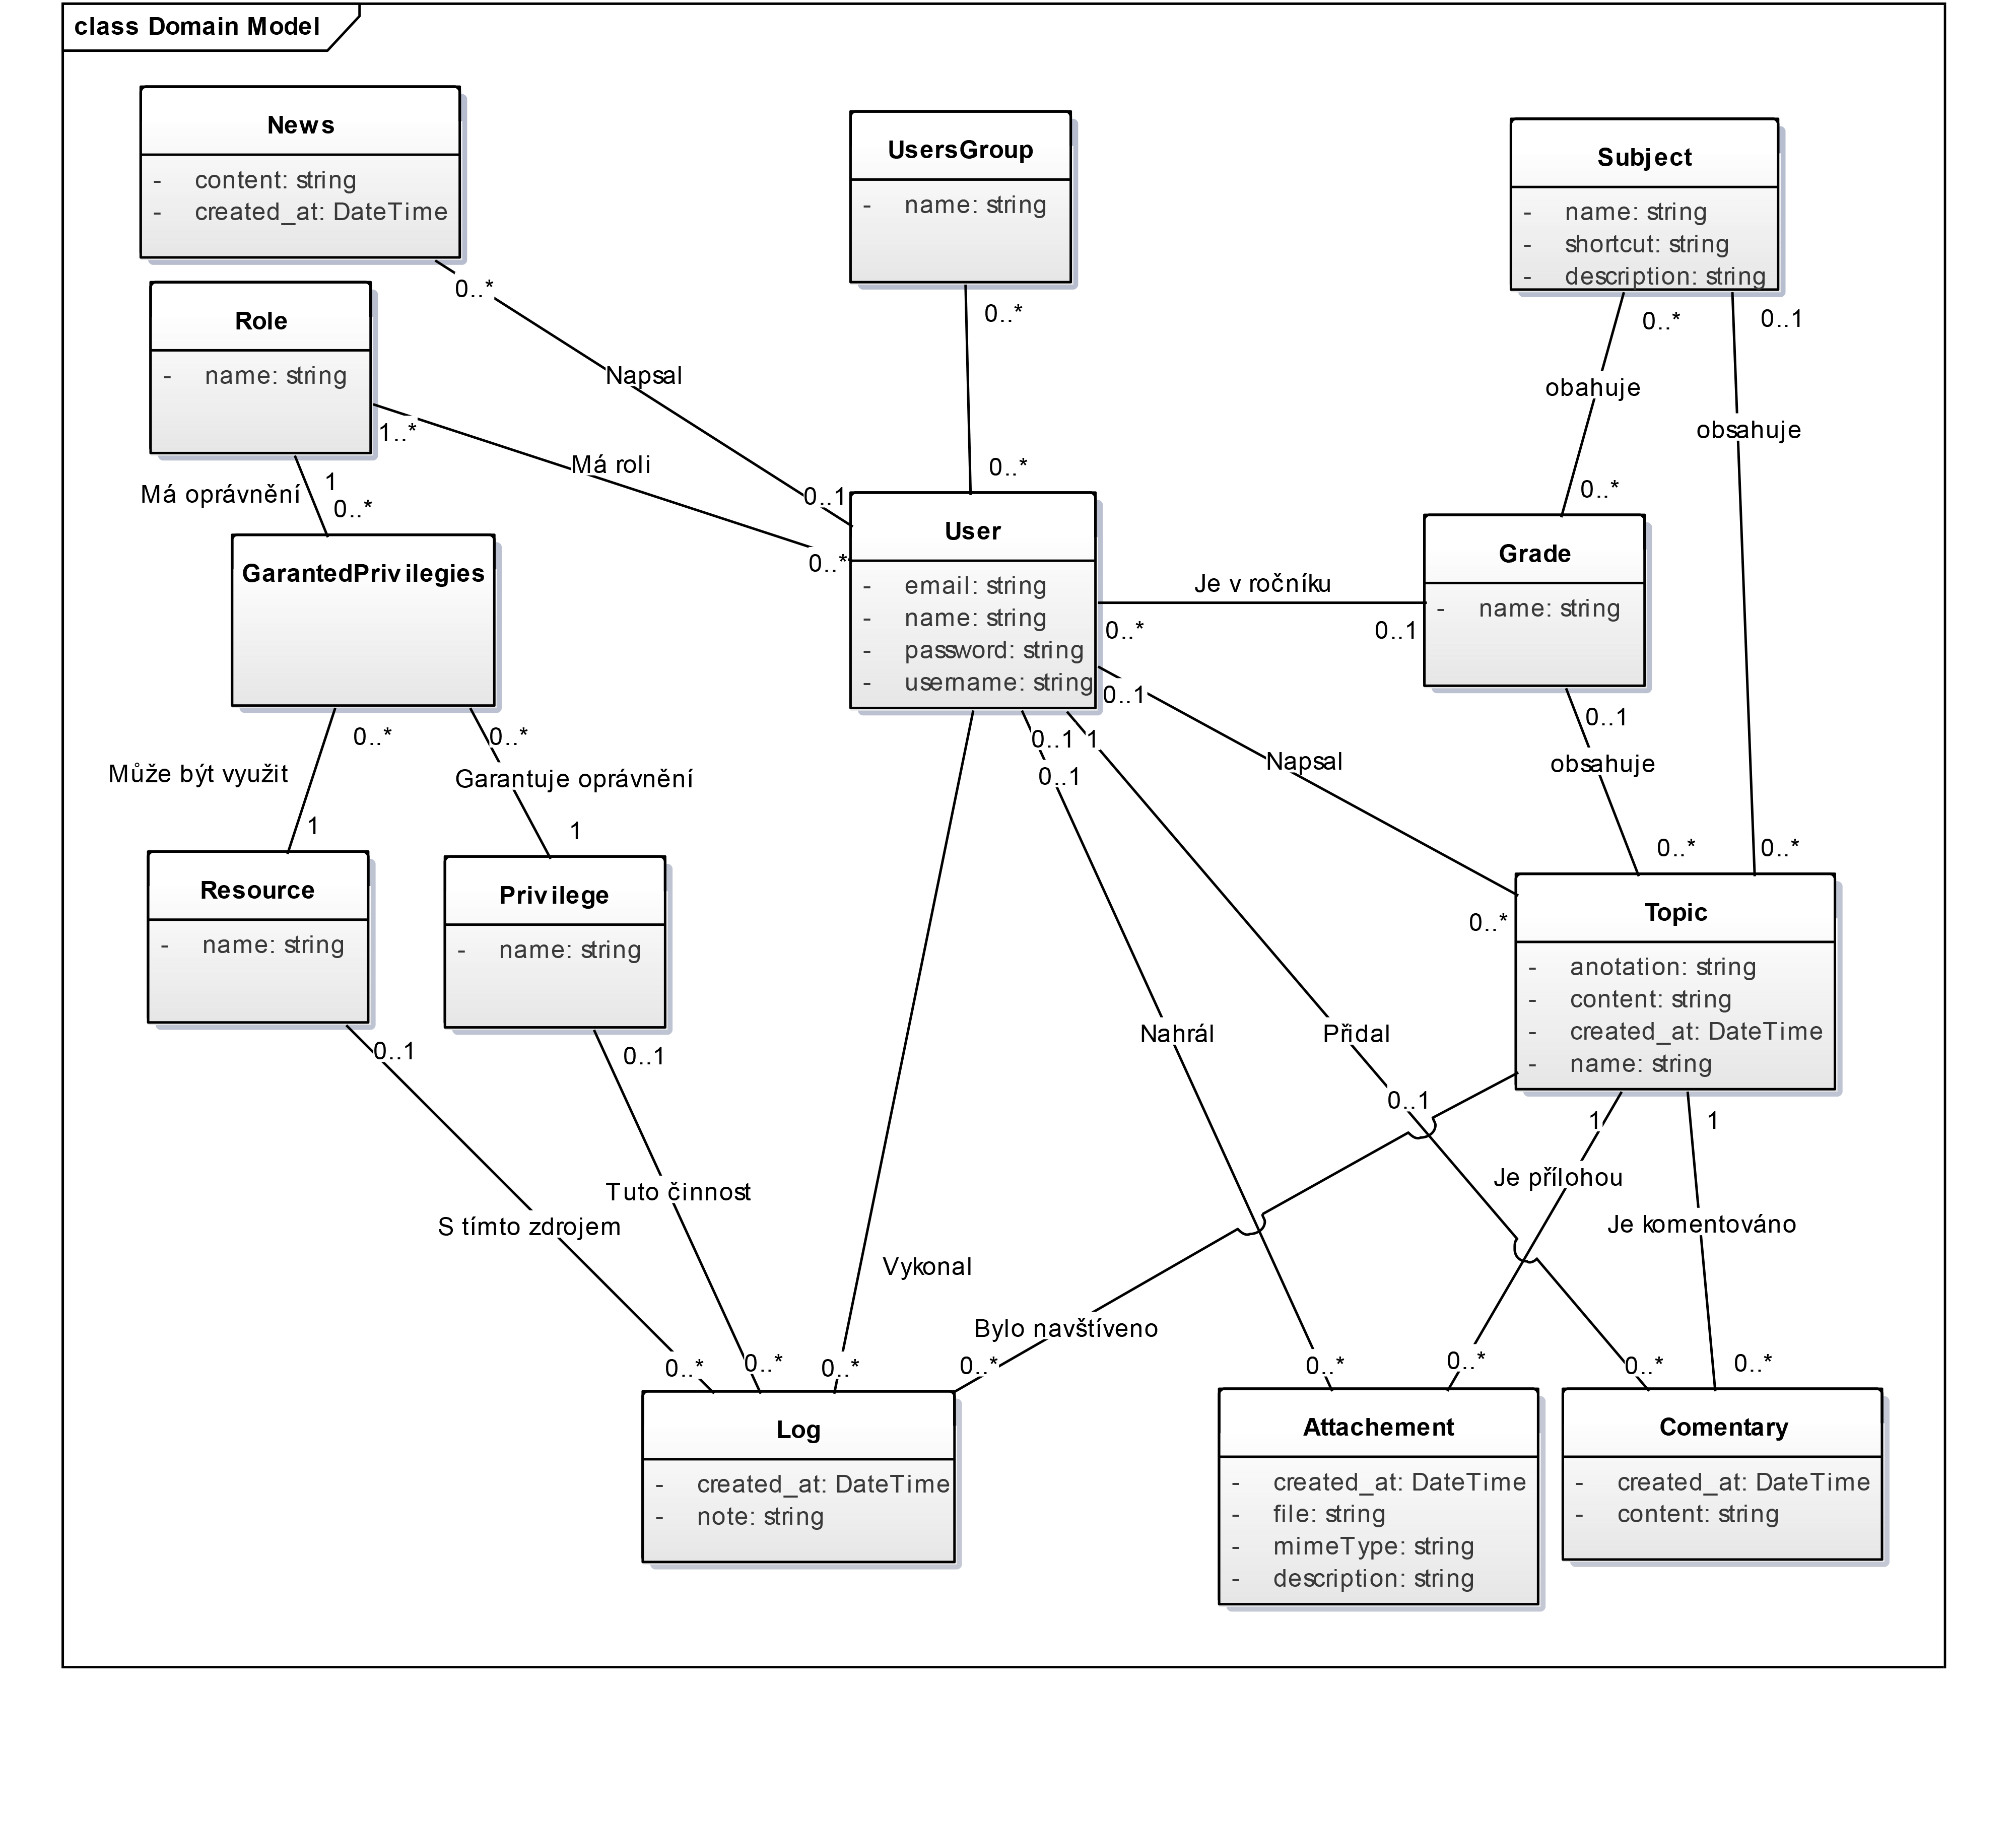
\includegraphics[scale=0.8]{domain_model.png}
	\caption{Diagram doménového modelu.} \label{fig:domainmodel} 
\end{figure}

\begin{center}
\end{center}

Doménový model může být logicky rozdělit na několik částí - uživatel a jeho oprávnění, materiály, log a novinky. Uživatel může být zařazen v různých skupinách, má svoji roli a s ní související oprávnění provádět dané operace nad určitými zdroji. Materiály se dají dobře třídit podle témat. Téma je zařazeno pod ročník a předmět. Každé téma může obsahovat řadu příloh a komentářů. U tématu, komentáře i přílohy je vlastník. V logu je zaznamenáno vše, co se na webu dělo a získaná data lze využít jako podklad pro statistiku. Log zaznamenává především návštěvy jednotlivých témat, ale i jiné operace s různými zdroji. Nakonec novinky, které jsou proudem zpráv od učitelů na hlavní stranu nebo automaticky generovanými oznámeními.

\section{Role a oprávnění}

Portál obsahuje řadu oprávnění a rolí. Systém oprávnění není nijak zvlášť složitý. Každá další role může o něco víc než ta předcházející. Tady je tedy seznam rolí a k nim přiřazených oprávnění.

\begin{itemize}
	\item Guest (nepřihlášený uživatel)
	\begin{itemize}
		\item formulář k přihlášení
		\item kontakt na současné administrátory webu
	\end{itemize}
	
	\item Zablokovaný účet
	\begin{itemize}
		\item vše co Guest
		\item má vlastní uživatelské jméno a heslo
	\end{itemize}

	\item Prohlídka
	\begin{itemize}
		\item vše co Zablokovaný účet
		\item může prohlížet jednotlivá témata
		\item nastavení svého účtu
		\item zobrazení vlastních statistik a hrubých statistik témat
	\end{itemize}

	\item Žák
	\begin{itemize}
		\item vše co Prohlídka
		\item může přidávat komentáře
		\item správa vlastních komentářů		
	\end{itemize}

	\item Učitel
	\begin{itemize}
		\item vše co Žák
		\item přidávání, editace, mazání témat (včetně příloh)
		\item správa diskuzí pod tématy
		\item správa uživatelských skupin
		\item odesílání newsletteru
		\item 	správa novinek
	\end{itemize}

	\item Administrátor
	\begin{itemize}
		\item všechna oprávnění
		\item správa účtů a skupin
		\item správa ročníků a předmětů
		\item zobrazení podrobných statistik
	\end{itemize}
\end{itemize}

Realizace oprávnění v systému proběhne dle následujícího schématu. Viz obrázek \ref{fig:permission}.

\begin{figure}
  \centering
	
\includegraphics[scale=0.45]{realizace_opravneni.png}
	\caption{Realizace oprávnění.} \label{fig:permission} 
\end{figure}

Než se provede operace, dojde nejprve k dotazu, zda ji může daný uživatel nad daným zdrojem provést. Rozhodování proběhne na základě role. Pokud je oprávněn danou operaci uskutečnit, bude provedena a uživatel bude dál pokračovat. Při zamítnutí je uživatel navrácen na poslední stránku a je mu oznámeno, proč nebylo možné operaci provést. Administrátor má povolení vždy nezávisle na systému rolí načítaném z databáze.

\subsection{Statistika}

Statistiky jsou u témat, jen jako přibližný počet návštěv v posledním týdnu a měsíci. Každý si může zobrazit vlastní statistiku ve svém profilu. Podrobné statistiky (kdo, kdy a které stránky navštěvuje) vidí pouze administrátor.


\section{Objektový návrh}
Každý presenter může být vykreslen řadou šablon podle použití. Viz obrázek \ref{fig:presentery}.

\begin{figure}
  \centering
	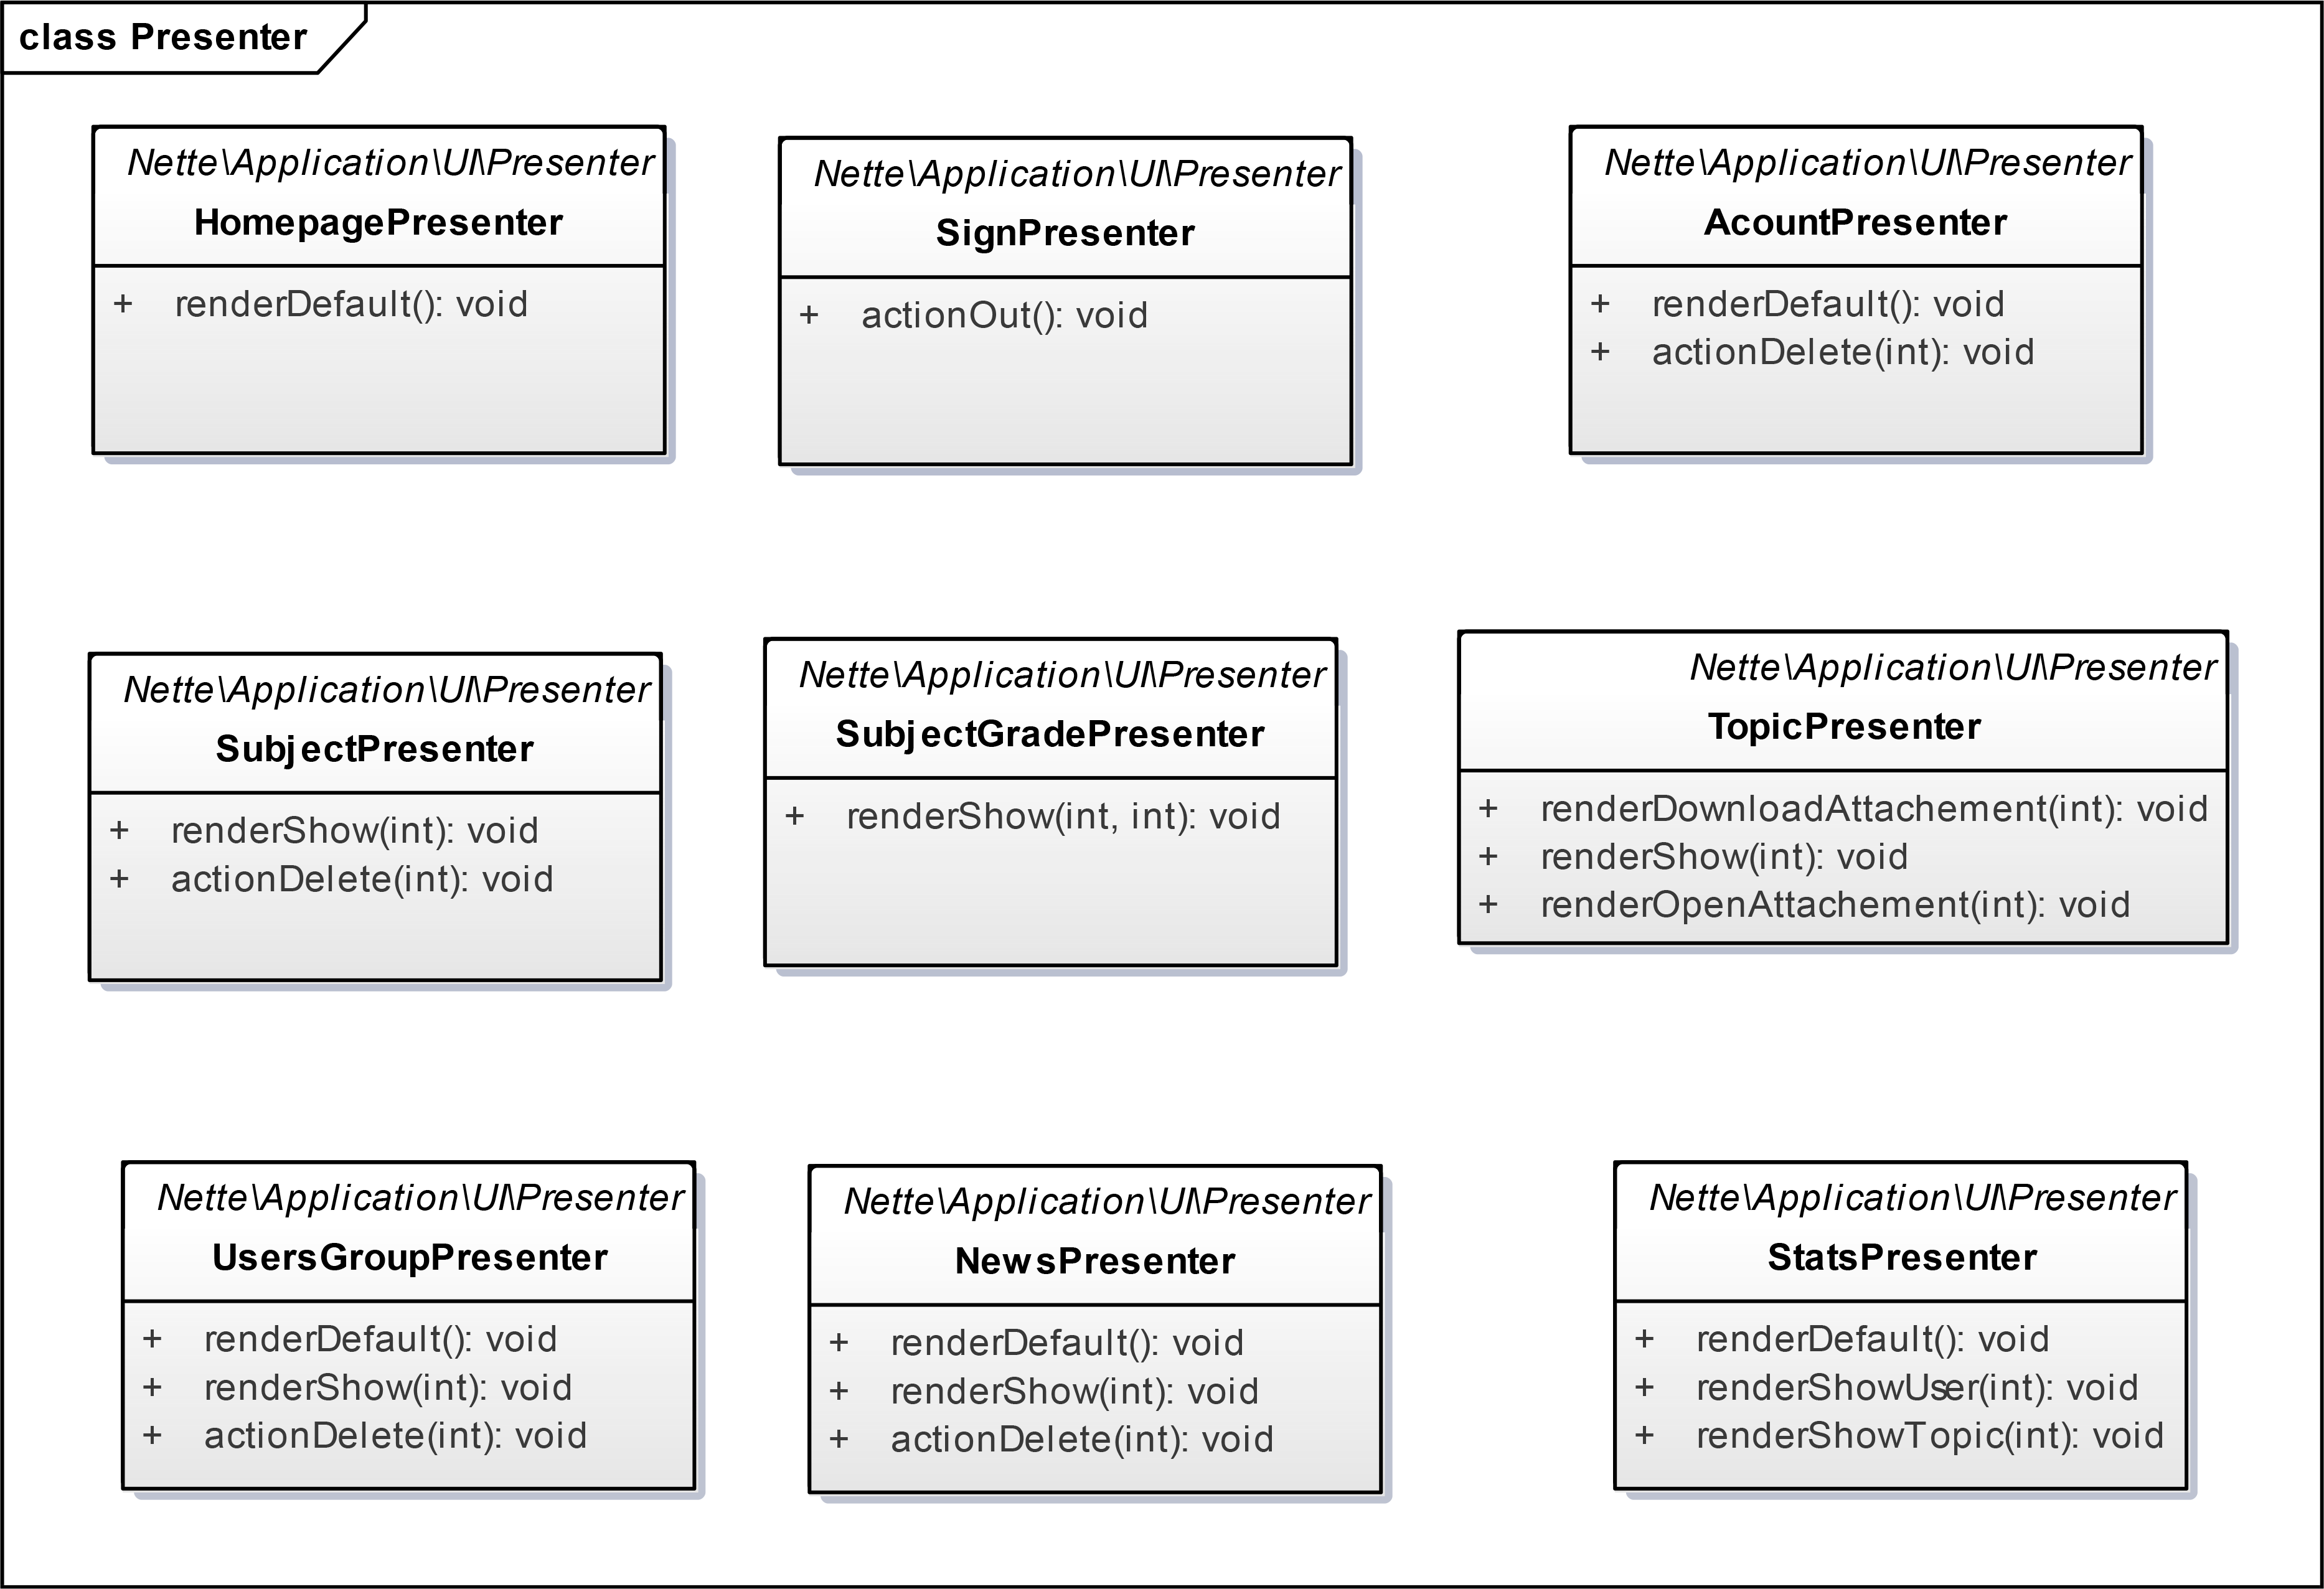
\includegraphics[scale=0.8]{presentery.png}
	\caption{Diagram presenterů.} \label{fig:presentery} 
\end{figure}

Každý presenter zodpovídá za sadu funkcí poskytovaných uživateli. V Nette každý presenter dědí od BasePresenteru. V tomto diagramu nepopisuji formuláře. HomepagePresenter je hlavní stránka. Tento presenter zodpovídá za možnost se přihlásit a zobrazení domovské stránky webu. SignPresenter je přihlášení. AcountPresenter obsahuje správu účtu. SubjectPresenter zobrazuje předmět. SubjectGradePresenter zobrazuje témata vybraného ročníku v předmětu. TopicPresenter obstarává vše okolo jednoho tématu. UsersGroupPresenter je správa skupin uživatelů. NewsPresenter umožňuje vkládání a odstraňování novinek a nakonec StatsPresenter, skrze který nahlížíme do statistik.

Ke presenterům existují šablony, přes které se vykresluje obsah. Neboť je jejich výčet silně závislý na implementaci, popíšu jejich seznam genericky. Každá funkce render v presenterech, která generuje webovou stránku, má svojí šablonu.

\chapter{Realizace}

Realizace probíhá formou psaní aplikace ve vývojovém prostředí. Neboť vyvíjím aplikaci sám, mohu si dovolit tvořit jednotlivé části a funkcionalitu v pro mě pohodlném pořadí.

V minulosti se mi osvědčil vývoj od databáze směrem nahoru, tedy až po frontend. Jakmile dobře funguje zobrazování dat z databáze uživateli, rozšiřuji svou aplikaci do šířky, přidávám funkce, a možnosti. Ve chvíli, kdy je aplikace stabilní a lze ji použít pro účel zadavatele, tak se ji snažím zároveň udržovat i online, abych měl rychlou zpětnou vazbu. Nakonec provádím import dat uživatele, abych tuto dlouhou a náročnou práci nedělal zbytečně vícekrát.

\section{Použité technologie}

Jazyky: PHP/Nette, MySQL, JavaScript, HTML, CSS. PHP/Nette na serverovou a logickou část aplikace. MySQL pro práci s databází, JavaScript pro řešení logiky na straně klienta, HTML pro obsah webových stránek a CSS pro visuální stránku.

Uložiště: MySQL/InnoDB, souborový systém. Relační databáze pro ukládání textových informací a souborový systém pro uložení nahraných souborů.

Externí balíčky: TinyMCE. Tento balíček pomocí JavaScriptu promění běžné textově pole na plně funkční WYSIWYG editor.

\section{Postup}

\subsection{Příprava databáze}

Z návrhu v Enterprise Architect jsem vygeneroval zakládací skripty pro databázi. Poté co byl skript vykonán jsem zkontroloval databázi, zda je v pořádku a doplnil do ní první testovací data - především prvního uživatele.

\subsection{Autentifikace a autorizace uživatele}

Nette framework nabízí vlastní řešení autentifikace a autorizace uživatelů, které se dá velmi snadno rozšířit. Základní myšlenku ověření uživatele jménem a heslem s porovnáním do vlastní databáze jsem rozšířil o uživatelské role a jednotlivá oprávnění.

\subsection{Struktura předmět, ročník a téma}

Podle návrhu jsem pokračoval v tvorbě presenterů a šablon. Přidal jsem presentery a Latte šablony, aby se dala data z databáze prohlížet uživatelsky přívětivou cestou.

\subsection{Komentáře}

Jedním z požadavků je diskuze pod jednotlivými tématy. Rozhodl jsem se pro implementaci, kde je možné v diskuzi dopovědět na vybraný komentář. S komentáři jsem vytvořil první interakci se systémem, která umožňuje vkládání nových dat.

\subsection{Přílohy}

Ke každému tématu kromě textu lze nahrát i množství příloh. Rozhodl jsem se pro zvýšení bezpečnosti neumožnit stažení souboru bez přihlášení.

\subsection{Přiřazení oprávnění}

Uživatelé v různých rolích mohou provádět různé operace. Například žáci nemohou upravovat témata. Naplnil jsem tabulku přiřazených oprávnění a implementoval jejich kontrolu před operace.

\subsection{Správa témat}

Aby mohli učitelé s webem pracovat, musí jim web umožňovat editaci. Těm, kteří mají oprávnění editovat témata jsem přidal malé ikonky editací a přidávání témat. K tématům jsem dodělal editační formuláře a logiku v aplikaci.

\subsection{Správa předmětů}

Přestože nabídka předmětů se na škole příliš měnit nebude, bylo by pošetilé nenechat školu samotnou, aby si mohla nabídku upravovat. Tomu, kdo má právnění, jsem přidal malé ikonky editace a přidávání předmětů. Udělal jsem formuláře, kde se upravuje které ročníky mají jaké předměty.

\subsection{Správa účtu}

Uživatel se může podívat na nějaké informace o sobě samém a měl by mít možnost si změnit heslo. Přidal jsem odkazy k zobrazení vlastního účtu a formulář k editaci. Zároveň jsem umožnil zobrazit všechny účty a kterýkoliv upravit.

\subsection{Správa skupin uživatelů}

Uživatelé se dělí do skupin. Důvod ke skupinám je newsletter. Přidal jsem tedy  odkaz na správu skupin. Udělal jsem formulář na přidání nové skupiny a editace stávajících.

\subsection{Newsletter}

Učitelé mohou svým žákům rozesílat hromadně zprávu. Žáky mohou filtrovat dle skupin. Nebo lépe oprávnění uživatelé mohou použít hromadnou poštu. Přidal jsem odkaz na odesílání hromadné pošty. Udělal jsem formulář včetně výběru skupin. tato funkce bude otestována až na produkčním serveru.

\subsection{Log a statistiky}

Abych mohly být na webu zobrazovány statistiky, je nutné nejprve logovat. Připravil jsem si funkci v modelu. Dopsal jsem její zavolání do renderování tématu a většiny akcí webu. Přidal odkaz na stránku souhrnných statistik. Ke každému tématu jsem přidal ikonku statistik, která vede na podrobné statistiky tématu. Podobnou ikonku jsem přidal i do uživatelského účtu, ta odkazuje na statistiky uživatele. A jsem nakonec umístil odkazy na statistiky uživatelů do seznamu všech uživatelů ve správě účtů.

\subsection{Design}

Přestože design mě skutečně baví, nechal jsem si ho nakonec. Zarovnal jsem prvky na stránkách a vyřešil barevnost.

\section{Testování}

V rámci testování bylo vyzkoušeno otevírání stránek témat, přidávání komentářů, přidávání témat, přihlašování a odhlašování. Vše je spouštěno na localhost a v debug režimu. Produkční server je výkonnější, lépe nastavený a stránky na něm poběží rychleji. Tabulka \ref{table:tests} ukazuje časy generování stránek a operací v milisekundách. Min ukazuje nejrychlejší vygenerování během deseti testů, Průměr je průměrná doba operace. Sloupec paměť ukazuje paměťovou náročnost stránky v MB. Databáze je čas potřebný k získání dat z databáze.

\begin{table}
\centering
\begin{tabular}{| p{5cm} | c | c | c | c |}
  \hline
    \bfseries Operace & \bfseries Min & \bfseries Průměr & \bfseries Paměť & \bfseries Databáze \\
    \hline \hline

   Otevření tématu (krátký text, jedna příloha, 4 komentáře) & $58 ms$ & $66 ms$  & $7,7 MB$ & $4,1 ms$ \\
   \hline
   Přidání komentáře & $46ms$ &$ 51ms$  & $6,7MB$ & $1,3ms$ \\
   \hline
   Přidání téma (krátký text, 1xPDF 836kB, 1x obrázek 82kB) & $68ms$ &$ 70ms$  & $7,1MB$ & $3,0ms$ \\
   \hline
   Zobrazení homepage (1x novinka) & $42ms$ &$ 45ms$  & $6,1MB$ & $1,6ms$ \\
   \hline
   Přihlášení & $136ms$ &$ 145ms$  & $6,5MB$ & $0,7ms$ \\
   \hline
   Odhlášení & $33ms$ &$ 34ms$  & $5,0MB$ & $0ms$ \\

\hline    
\end{tabular}
\caption[Rychlost operací na webu.]{Rychlost generování stránek a operací na webu.}
\label{table:tests}
\end{table}

Testování rychlosti ukázalo, že framework zpomaluje generování stránek. Menší rychlost by měla být vyvážena vyšší bezpečností a jednodušším rozšiřováním i udržováním aplikace.

Testování funkčnosti probíhalo po celou dobu vývoje a případné funkční chyby budou nahlášeny a vyřešeny.

\section{Nasazení}

Nasazení je naplánované na leden 2015. V rámci nasazení je třeba přenést stávající materiály.

\section{Screenshoty}

Následující snímky obrazovky ukazují jednu běžnou stránku (viz. obrázek \ref{fig:screenshot1}) a přípravu nového téma (viz. obrázek \ref{fig:screenshot2}). Nasazená aplikace může mít odlišný design.

\begin{figure}
  \centering
	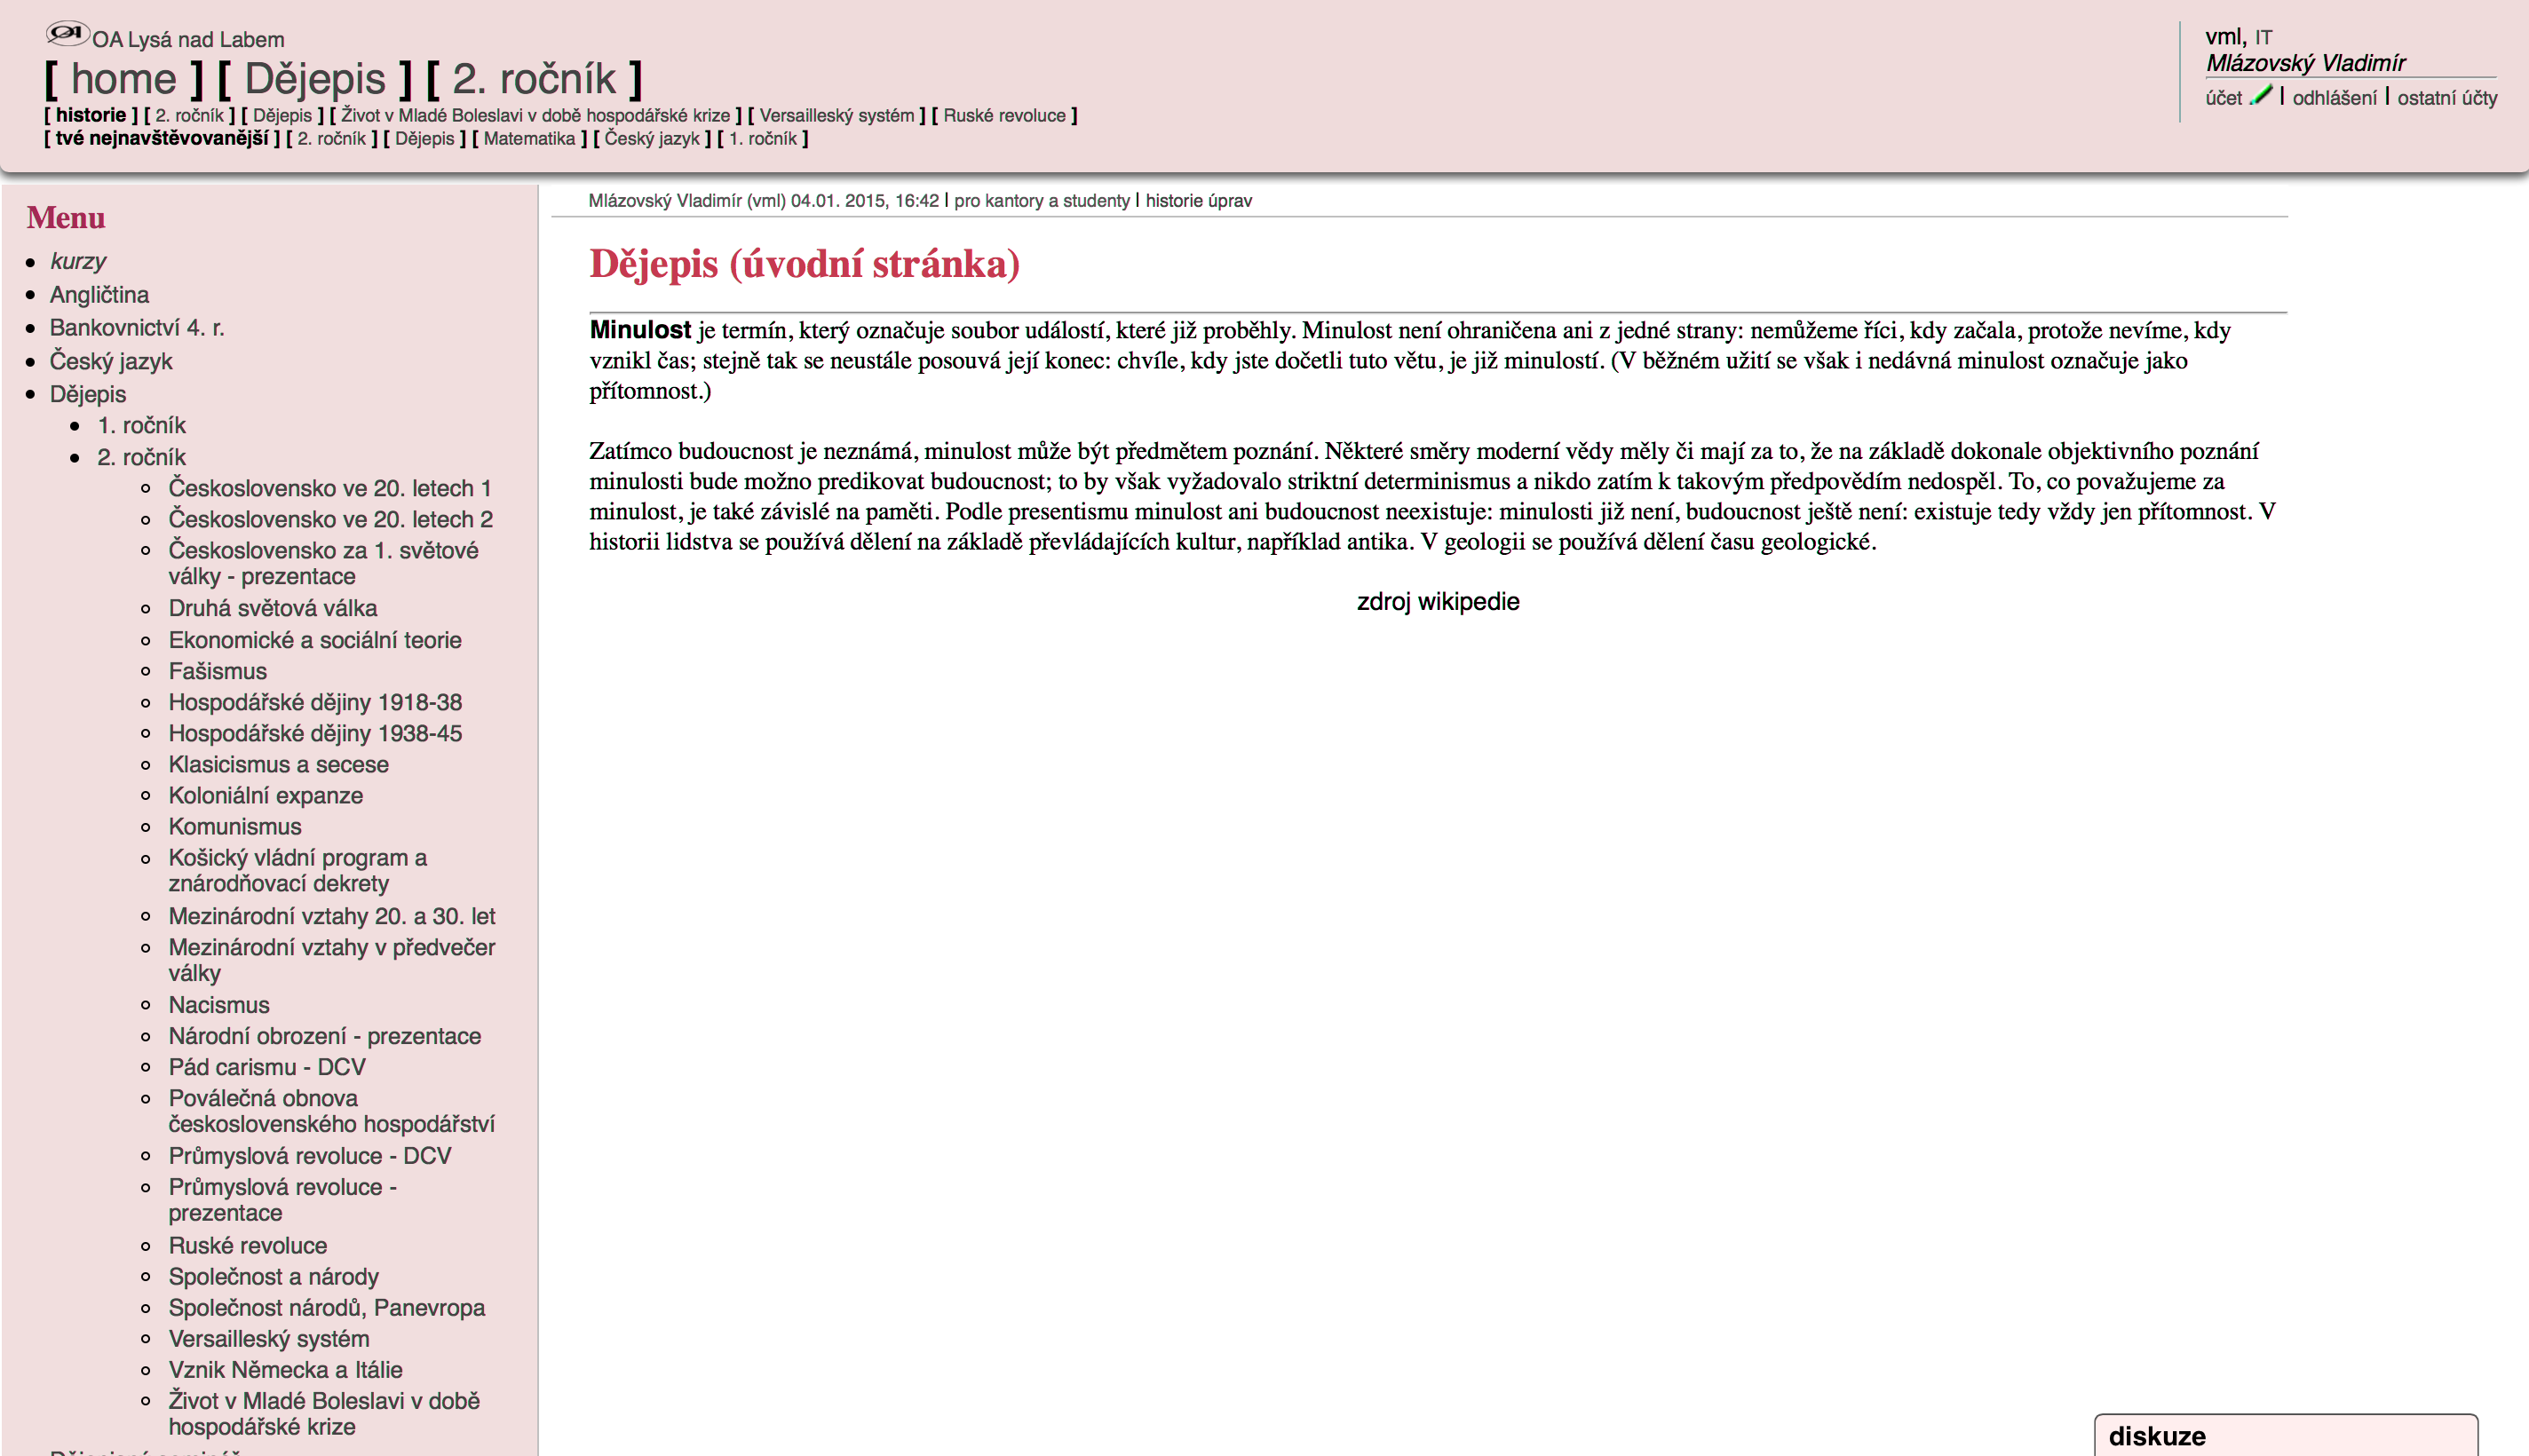
\includegraphics[scale=0.24]{screenshot1.png}
	\caption{Úvodní stránka předmětu dějepis.} \label{fig:screenshot1} 
\end{figure}


\begin{figure}
  \centering
	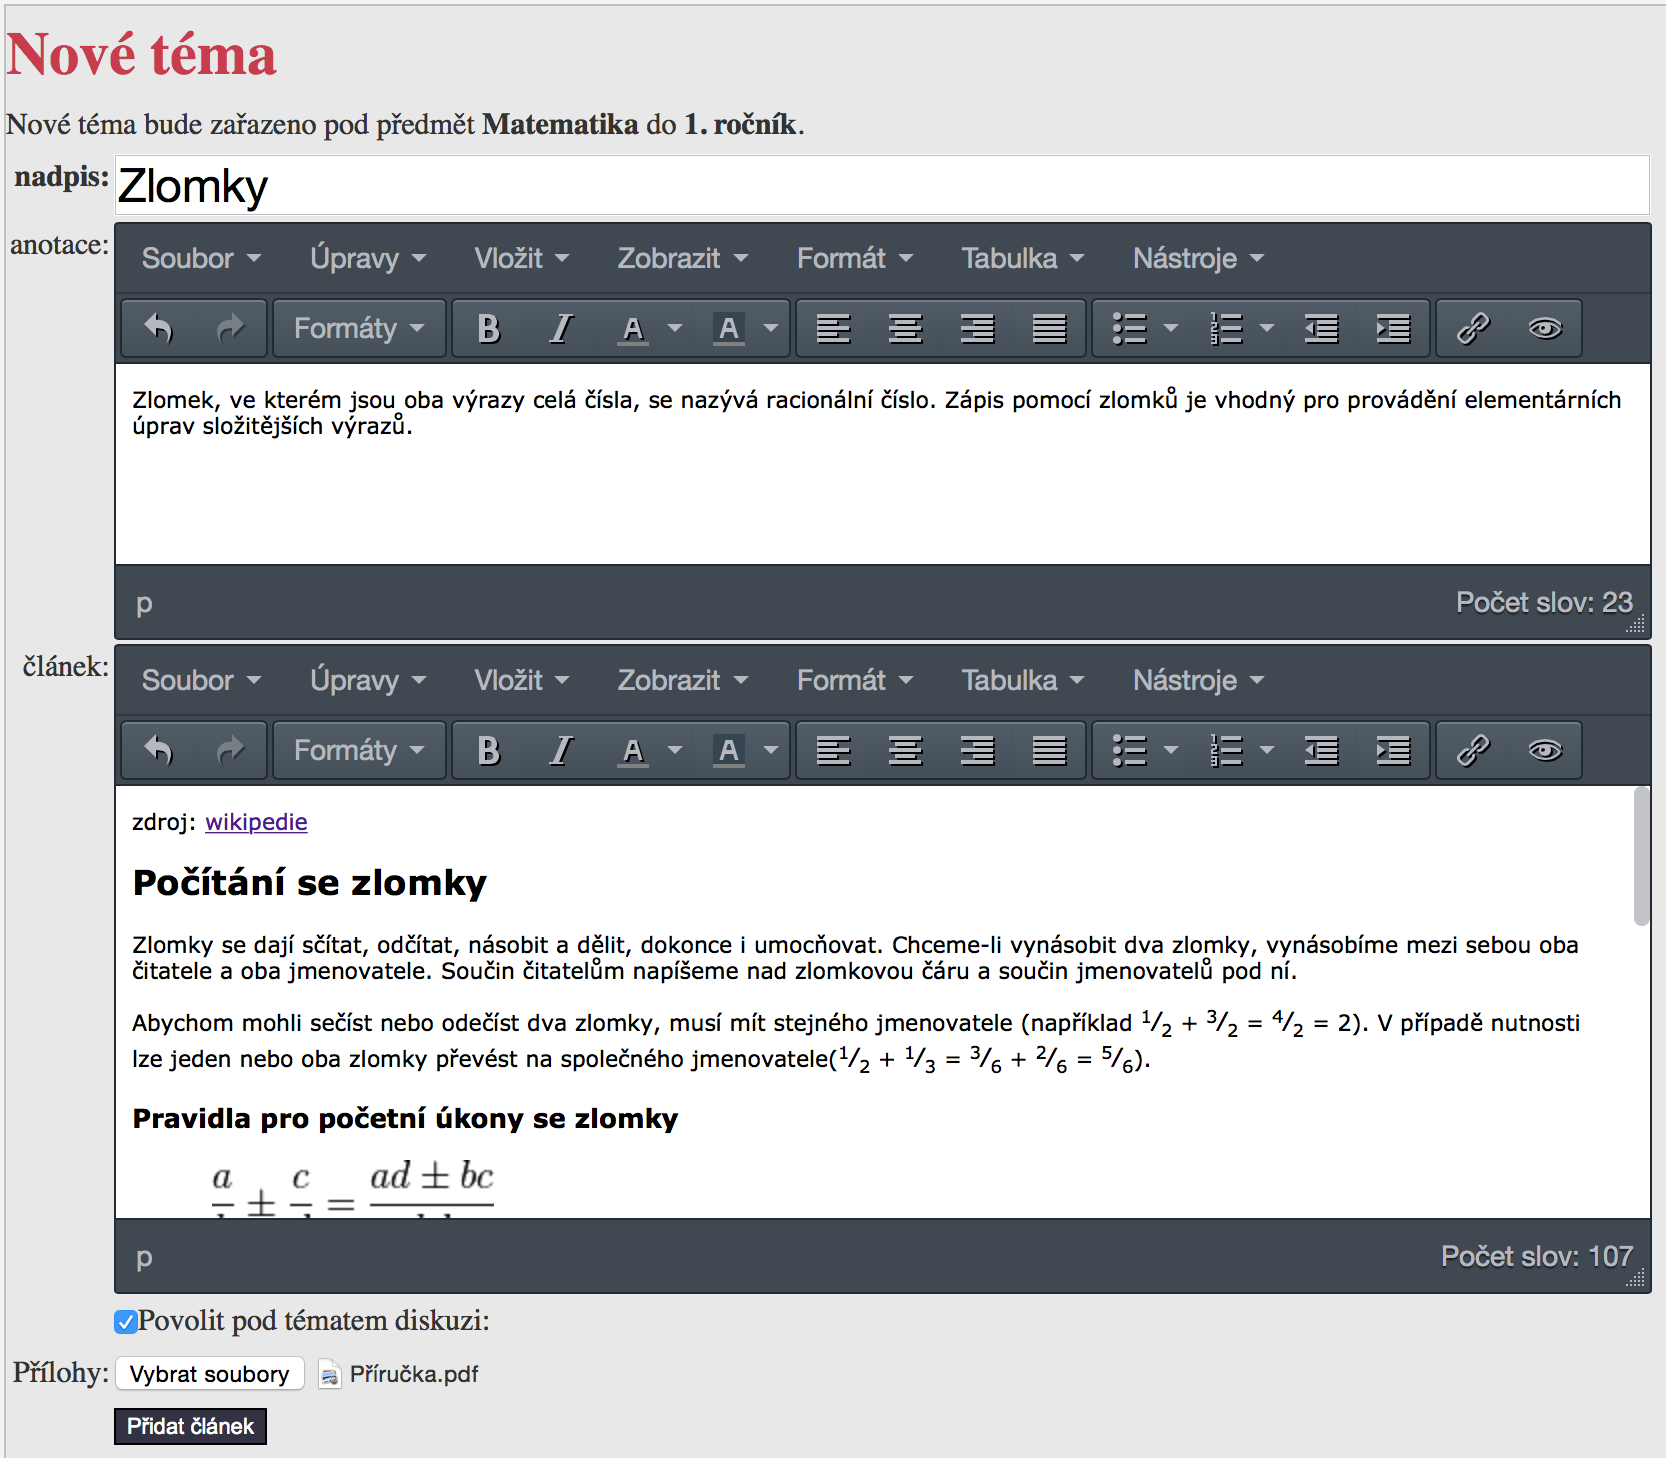
\includegraphics[scale=0.4]{screenshot2.png}
	\caption{TinyMCE vytvoření nového téma.} \label{fig:screenshot2} 
\end{figure}



\begin{conclusion}
Během ledna přechází škola na tento nový systém. Až zpětná vazba ukáže skutečný výsledek mé práce. Protože jsem vyšel vstříc požadavkům zadavatele a systém výrazně zjednodušil, očekávám dobré výsledky.
	
Funkční požadavky byly splněny. Na webu existují všechny role, pevná hierarchie menu editor podobný Wordu, možnost nahrávání příloh, rozesílání hromadné pošty, záznam návštěv a je možné pod tématy rozvádět diskuze.

Webový portál byl skutečně naprogramován v PHP/Nette a poběží na stejné doméně (i serveru) jako prezenční web školy. K materiálům se dá skutečně dostat jen jako přihlášený uživatel.

Do budoucna bych rád do webu dodělal ještě jednu roli, ta by umožňovala vybraným studentům spolupracovat na tvorbě webu. Navíc bych rád systém nabídl i na jiných malých středních školách. Sdílení materiálů mezi školami byla hezká myšlenka, ale nemá příliš smysl něco takového budovat. Dále bych rád umožnil v systému zaznamenávat dosažené výsledky podobně jako se to dá v bakalářích. Mít známky online je praktické a jedno celoškolské řešení zní jako dobrý nápad.

Čas ještě ukáže, jaké funkce se budou hodit. Očekávám, že přidám ještě dávkové zpracování nových žáků, automatický přesun mezi ročníky.

Přepsání webu byla pro mě velká zkušenost. Je to první systém, který jsem postavil nad  frameworkem. Nebylo to jednoduché, ale mám konečně větší web, který je mým dítětem a mohu se s ním reprezentovat při získávání dalších zakázek nebo zaměstnání. 

\end{conclusion}




\bibliographystyle{csn690}
\begin{thebibliography}{9}

\bibitem{moodle}
FOSTER, Helen. Features. MOODLE. \textit{Features} [online]. 2014, 2014-07-09 [cit. 2014-12-04]. Dostupné z:\\ \url{https://docs.moodle.org/28/en/index.php?title=Features&oldid=113496}

\bibitem{pnovotny}
	NOVOTNÝ, Petr. \emph{Soukromá konzultace}. 2014-11-13, Praha. Programátor ze slever.cz\\

\bibitem{edux}
	Kadlec, Tomáš. EDUX, PřiŘíz a další. EDUX. \textit{EDUX, PřiŘíz a další} [online]. 2012, 2012-10-24 [cit. 2014-12-04]. Dostupné z:\\ 
	\url{https://edux.fit.cvut.cz/prezentace/2012-10-24}
	
\bibitem{nette}
	NETTE FOUNDATION. \textit{Dokumentace} [online]. 2014 [cit. 2014-12-04]. Dostupné z:
	\url{http://doc.nette.org/cs/2.2/}\\

\bibitem{dokuwiki}
DokuWiki. GOHR, Andreas. \textit{DokuWiki} [online]. 2014, 2014-05-07 [cit. 2014-12-04]. Dostupné z: \\
\url{https://www.dokuwiki.org/cs:dokuwiki}

\bibitem{phpfashion}
Hackeři vám zaútočí na web. GRUNDL, David. \textit{phpFashion} [online]. 2014, 2009-07-02 [cit. 2014-12-04]. Dostupné z:\\
\url{http://phpfashion.com/hackeri-vam-zautoci-na-web}

\end{thebibliography}


\appendix

\chapter{Seznam použitých zkratek}
% \printglossaries
\begin{description}
	\item[CSS] Cascading Style Sheets
	\item[HTML] HyperText Markup Language
	\item[MB] MegaByte - 1048576 bajtů
	\item[MVC] Model View Controller
	\item[OA] Obchodní akademie
	\item[PDF] Portable Document Format
	\item[PHP] PHP: Hypertext Preprocessor
	\item[SQL] Structured Query Language
	\item[TUR] Tvorba uživatelského rozranní
	\item[WYSIWYG] What you see is what you get
\end{description}

\chapter{Repositář}

%upravte podle skutecnosti

Celý projekt žije v github repositáři. Ten se dá prohlédnout na adrese:

\begin{center}
 \url{https://github.com/mlazovla/oalysa}
\end{center}
 
 Repositář může být stažen jako komprimovaná složka ZIP nebo naklonován pomocí git.

\begin{figure}
	\dirtree{%
		.1 design.\DTcomment{složka s návrhem}.
		.2 DDL.SQL\DTcomment{Zakládací skripty pro databázi.}.
		.1 implementace\DTcomment{složka s aktuální implementací}.
		.1 bc\DTcomment{bakalářská práce}.
		.2 thesis.tex\DTcomment{zdrojová forma práce ve formátu \LaTeX{}}.
		.2 thesis.pdf\DTcomment{text práce ve formátu PDF}.
		.2 thesis.ps\DTcomment{text práce ve formátu PS}.
		.1 nasazeni.txt\DTcomment{jak nasadit aplikaci}.
	}
\end{figure}

\chapter{Příručky}

\section{Uživatelská příručka}

Vítejte ve webovém portálu na podporu výuky Vaší školy. Pro používání webu je nutné se přihlásit svým uživatelským jménem a heslem. Tyto údaje obdržíte od svého učitele nebo od administrátora webu.

\subsection{Jsem žák}

Přestože se mnoho žáků navzájem obohacuje skrz sociální sítě a tento web pak vypadá jako slabá konkurence, není to pravda a obě služby se doplňují. Když sociální sítě umožňují rychlou komunikaci a výměnu posledních novinek. Tento web pak slouží jako \textbf{přehledný archiv} probírané látky z oficiálního zdroje vlastní školy.

Jako žák můžete prohlížet na webových stránkách veškerý obsah a většinu témat komentovat, ptát se spolužáků či vyučujících a zanechat tak zpětnou vazbu k probírané látce pro ostatní.

Po přihlášení si zvolte v levé části předmět a ročník, ve kterém se látka vyučuje. V menu zvolte téma, které odpovídá vaším preferencím. Téma se skládá z textového popisu a příloh dříve nahraných Vaším vyučujícím. Pod přílohami je diskuze, tam se dají položit dotazy k tématu a nalézt odpovědi na nejasné části probírané látky.

Po načerpání znalostí se můžete odhlásit v pravém horním rohu nebo stačí zavřít okno prohlížeče, účet bude automaticky odhlášen během několika minut.

Změnu údajů o svém účtu můžete provést na záložce účet vpravo nahoře. Lze změnit heslo, email, zapnout či vypnout newsletter.

\subsection{Jsem učitel}

Učitelé se často spoléhají na literaturu a knižní zdroje, ale ve druhé dekádě 21. století byly knihy jednoznačně překonány. Nevím zda obsahem, ale jednoznačně formou. Papír nenabídne takovou míru interaktivity a ,to především, možnost vyhledávání. Tento web umožňuje komunikaci s Vašimi žáky na nové rovině a ti, kteří se chtějí vzdělávat, budou zdejší obsah konzumovat.

Jako učitel můžete, stejně jako Vaši žáci, procházet web, pročítat si jej a diskutovat pod tématy, dávat svým žákům odpovědi. Navíc pro ně můžete vytvářet materiály. Přidávat témata, nahrávat k nim přílohy. Díky uzavřenému systému můžete svým žákům poskytovat libovolné materiály, které by jim mohly být poskytnuty ve škole.

Hlavním úkolem učitele je na tomto webu udržovat právě probíranou látku aktuální a zanechávat žákům dostatek informací k řešené problematice, aby se mohli věnovat škole i v pohodlí domova a mohli se lépe připravit. Není cílem na webu udržovat všechno. Web by měl být odrazovým můstkem, místem, kde se žák může podívat na prezentaci vyzkoušet si jednu variantu testu.

Každé \textbf{téma} obsahuje textovou část, přílohy a diskuzi. V textové části by měl být popis daného tématu a motivace ke studiu problematiky. V přílohách je nosná část - tedy podklady ke studiu a ukázkové testy. Diskuze slouží k dořešení nejasností.

\textbf{Vytvořit nové téma} můžete po kliknutí na předmět a ročník, ve kterém by se nové téma mělo nacházet. Tlačítkem plus v záhlaví menu přidáte do zvoleného předmětu pod zvolený ročník nové téma. Postupujte podle kroků ve formuláři.

Velmi podobně můžete témata upravovat. Po otevření tématu si povšimněte malé ikony tužky vedle názvu tématu. Tato ikonka slouží k \textbf{editaci aktuálního tématu}. Editace umožňuje změnit text, přidávat či mazat přílohy a spravovat diskuzi.

Web Vám umožňuje odeslat \textbf{hromadnou poštu}. Vybraným skupinám žáků můžete odeslat stejný email. Tím můžete žáky upozornit na případné změny na webu nebo rozeslat informace o plánované akci v rámci Vašeho předmětu.

Web zaznamenává aktivitu svých uživatelů. Můžete nahlédnout do souhrnných statistik a zjistit, zda jsou vámi vytvořené materiály prohlížené.

Změnu údajů o svém účtu můžete provést na záložce účet vpravo nahoře. Lze změnit heslo, email, zapnout či vypnout newsletter.

\chapter{Ukázka zdrojového kódu}

\section{Model}

Třída obstarávající přístup k rolím.
\begin{tiny}
\begin{verbatim}
/**
 * Třída obstarávající přístup do databázovou tabulku s údaji o jednotlivých Rolích.
 * Převzaté datové položky z databáze:
 *  - int id
 *  - varchar name
 *  - int inherit FK
 */
class Role extends \Nette\Database\Table\Selection {
    private $table = "Role";
    private $db;

    public function __construct(\Nette\Database\Context $database) {
        parent::__construct($database->getConnection(), $this->table,
            $database->getDatabaseReflection());
        $this->db = $database;
    }

    /**
     * Translate role name to role id.
     * @param string $role_name
     * @return int
     */
    public function roleName2id($role_name) {
        $res = $this->where('name', $role_name)->limit(1)->fetch();
        return $res['id'];
    }
    
    /**
     * Get list of all parent roles
     * 
     * @param mixed $role_id
     * @return array[int]{id, role_name}
     */
    public function getAllParents($role_id_or_id) {
        if (is_int($role_id_or_id))
            $role_id = $role_id_or_id;
        else
            $role_id = $this->roleName2id($role_id_or_id);
        
        $i = 0;
        while($role_id != null && $i < 10) {
            $i++;
            $role = new Role($this->db);
            $tmp = $role->where('id', $role_id)->limit(1)->fetch();
            $res[] = array('id' => $tmp['id'], 'name' => $tmp['name'],
                'role_id' => $tmp['role_id']);
            $role_id = $tmp['role_id'];
            unset($role);
        }
        return $res;
    }
}

\end{verbatim}
\end{tiny}
\pagebreak

\section{Presenter}

Třída obstarávající přístup a akce spojené s tématem. Zkráceno. 

\begin{tiny}
\begin{verbatim}

/**
 * Topic presenter.
 */
class TopicPresenter extends BasePresenter
{
    //--------------------------------------------------------
    // SHOW TOPIC
    
    public function __construct(Nette\Database\Context $database)
    {
        $this->database = $database;
    }

    /**
     * Prepare data to display one Topic (discusion, ...)
     * @param int $subjectId
     */
    public function renderShow($topicId)
    {        
        // Neopravneny uzivatel
        if (!$this->user->loggedIn ||
            !$this->user->isAllowed('topic','read')) {
            $this->flashMessage('Nemáte oprávnění číst články.',
                'warning');
            $this->redirect('Homepage:');
            return;
        }  
                
        $subject = new Subject($this->database);
        $grade = new Grade($this->database);
        $topic = new Topic($this->database);

        $this->template->subject = $topic->getSubject($topicId);
        $this->template->grade = $topic->getGrade($topicId);
        $this->template->topic = $topic->get($topicId);

        $gradeId = $topic->getGrade($topicId)->id;
        if ($gradeId == null) {
            $this->template->topics = null;
        }
        else {
            $this->template->topics = $topic
                ->where('Subject2Grade.grade_id', $gradeId);
        }
        
        if ($this->user->isAllowed('attachement', 'read')) {   
            /**
             * @var Attachement $attachement
             */
            $attachement = new Attachement($this->database);
            $this->template->attachements = $attachement->
               getByTopic($topicId);
        }
        
        if ($this->user->isAllowed('comentary', 'read')) {        
            /**
             * @var Comentary $comentary
             */
            $comentary = new Comentary($this->database);
            $this->template->comentaries = $comentary->
               getByTopic($topicId);
        }
        
        // Opravneni
        $this->template->isAllowedToWriteComents = $this->user
            ->isAllowed('selfComentary', 'insert');
        $this->template->isAllowedToDeleteSelfComent = $this->user
            ->isAllowed('selfComentary','delete');
        $this->template->isAllowedToDeleteAnyComent = $this->user
            ->isAllowed('comentary','delete');
        $this->template->isAllowedToDeleteAnyTopic = $this->user
            ->isAllowed('topic', 'delete');
        $this->template->isAllowedToDeleteSelfTopic = $this->user
            ->isAllowed('selfTopic', 'delete');
        
    }
    
     /**
     * Render attachement for safe download
     * @param int $attachementId
     */
    public function renderDownloadAttachement($attachementId) {
        if (!$this->user->isAllowed('attachement', 'read')) {
            $this->redirect('Homepage:');
            $this->flashMessage('Nemáte oprávnění číst přílohu článku.',
                'warning');
            return;
        }
        
        $attachement = new Attachement($this->database);
 
        $path = $attachement->getPathById($attachementId);
        $filename = $attachement->get($attachementId)->name;
        // For Gecko browsers mainly        
        header('Content-Transfer-Encoding: binary'); 
        header('Last-Modified: ' . $attachement->get($attachementId)
            ->created_at . ' GMT');
        // Allow support for download resume
        header('Accept-Ranges: bytes');
        header('Content-Length: ' . filesize($path));  // File size
        header('Content-Encoding: none');
        // Change the correct mime type
        header('Content-Type: ' . $attachement->get($attachementId)
             ->mimeType);
        // Make the browser display the Save As dialog
        header('Content-Disposition: attachment; filename=' . $filename);
        // finaly the file
        readfile($path);
        exit();
    }
    
     /**
     * Create form to comentary
     * @return form
     */
     protected function createComponentComentaryForm()
     {
        $form = new Nette\Application\UI\Form;
        $form->addTextArea('content', 'komentář:')
        ->setRequired();
        $form->addHidden('topic_id', $this->getHttpRequest()
            ->getQuery('topicId'));
        $form->addHidden('answer_on', null);
        $form->addSubmit('send', 'Komentovat');
        $form->onSuccess[] = $this->comentaryFormSucceeded;
    
        return $form;
    }

     /**
     * Solve the comentary form.
     * @param form
     */    
    public function comentaryFormSucceeded($form)
    {                
        $values = $form->getValues();
        
        $authorizator = new MyAuthorizator();
        $authorizator->injectDatabase($this->database);
        $this->user->setAuthorizator($authorizator);
        if (!$this->user->isAllowed('selfComentary', 'insert')) {
            $this->flashMessage('Nemáte oprávnění komentovat články.'
                ,'warning');
            $this->redirect('show', $values->topic_id);
            return;
        }
        
        $answer_on = (is_numeric($values['answer_on'])) ?
            $values['answer_on'] : null; 
        
        $comentary = new Comentary($this->database);
        $comentary->insert(
            array(
                'user_id' => $this->user->getIdentity()->id,
                'topic_id'=> $values['topic_id'],
                'content' => $values['content'],
                'comentary_id' => $answer_on
            )
        );
    
        $this->flashMessage("Komentář přidán.", 'success');
        $this->redirect('show', $values->topic_id);
    }
    
     /**
     * Delete coment by id
     * @param int $coment_id
     */    
    public function actionDeleteComent($coment_id) {
        $authorizator = new MyAuthorizator();
        $authorizator->injectDatabase($this->database);
        $this->user->setAuthorizator($authorizator);
        $coment = new Comentary($this->database);
        $owner_id = $coment->get($coment_id)->user->id;
        $topic_id = $coment->get($coment_id)->topic->id;
        if ($this->user->id == $owner_id) { // Vlastni komentar
            if (!$this->user->isAllowed('selfComentary', 'delete')) {
                $this->flashMessage('Nemáte oprávnění' 
                   .' odstranit vlastní komentář.','warning');
                $this->redirect('show', $topic_id);
            } 
            $coment = new Comentary($this->database);
            $coment->where('id', $coment_id)->delete(); 
            $this->flashMessage('Komentář byl odstraněn.');
            $this->redirect('show', $topic_id);     
        }
        else { // komentar libovolneho uzivatele
            if (!$this->user->isAllowed('comentary', 'delete')) {
                $this->flashMessage('Nemáte oprávnění mazat komentáře.'
                    ,'warning');
                $this->redirect('show', $topic_id);
                return;
            }
            $coment = new Comentary($this->database);
            $coment->where('id', $coment_id)->delete();
            $this->flashMessage('Komentář byl odstraněn.');
            $this->redirect('show', $topic_id);
        }
    }

};    

\end{verbatim}
\end{tiny}
\pagebreak

\section{Latte šablona}

Latte šablona vypisující komentáře. 

\begin{tiny}
\begin{verbatim}

<div id="comentaries">
    <h2>Komentáře</h2>
    {if $comentaries}
        {foreach $comentaries as $c}
            <div class="comentar">
                {if $c->comentary != null}
                <a name="comentary{$c->id}"></a>
                <div class="question">
                    <span class="user">{$c->comentary->user->name}</span>
                    <span class="date">{$c->comentary->created_at}</span>
                    <a href="#comentary{$c->comentary->id}" title="Ukázat komentář." 
                         class="buttonShow">Ukázat</a>
                    napsal: {$c->comentary->content|truncate:50}                    
                </div>
                {/if}
                <div class="answer">
                    <span class="user">{$c->user->name}</span>
                    <span class="date">{$c->created_at|date:'%d.%m.%Y %H:%M'}</span>
                    {if $isAllowedToWriteComents}
                        <a
                            class="buttonAnswer_on"
                            href="#comment"
                            title="Odpovědět"
                            onClick="
                                setInputValueById('frm-comentaryForm-answer_on','{$c->id}');
                                setElementValueById('answer_on_message', '{$c->content|truncate:30}');
                        ">Odpovědět</a>
                    {/if}
                    {if ($isAllowedToDeleteAnyComent || 
                        ($isAllowedToDeleteSelfComent && $c->user->id == $currentUser['id'])
                    )}
                        <a n:href="deleteComent $c->id" class="buttonDelete">X</a>
                    {/if}
                    <span class="content">{$c->content}</span>
                </div>
            </div>
        {/foreach}
    {else}
        <p>K tomuto tématu nejsou zatím žádné komentáře.</p>
    {/if}

\end{verbatim}
\end{tiny}


\end{document}
